\chapter{Background and motivation}
\label{chapter:background}

\section{Existing conceptual frameworks for sparse tensor accelerators}

This work builds on prior efforts to build conceptual frameworks around sparse tensor accelerators, which will be reviewed in this section.

All of the works in this section (except for Sparseloop\cite{sparseloop} itself) -  preceded Sparseloop, which introduced the term ``SAF''. Thus, any usage of the term ``SAF'' or ``SAF microarchitecture'' in this section is my own word choice and is not a quote.

\subsection{TACO\cite{taco_format} hierarchical sparse tensor formats}

\begin{figure}[H]
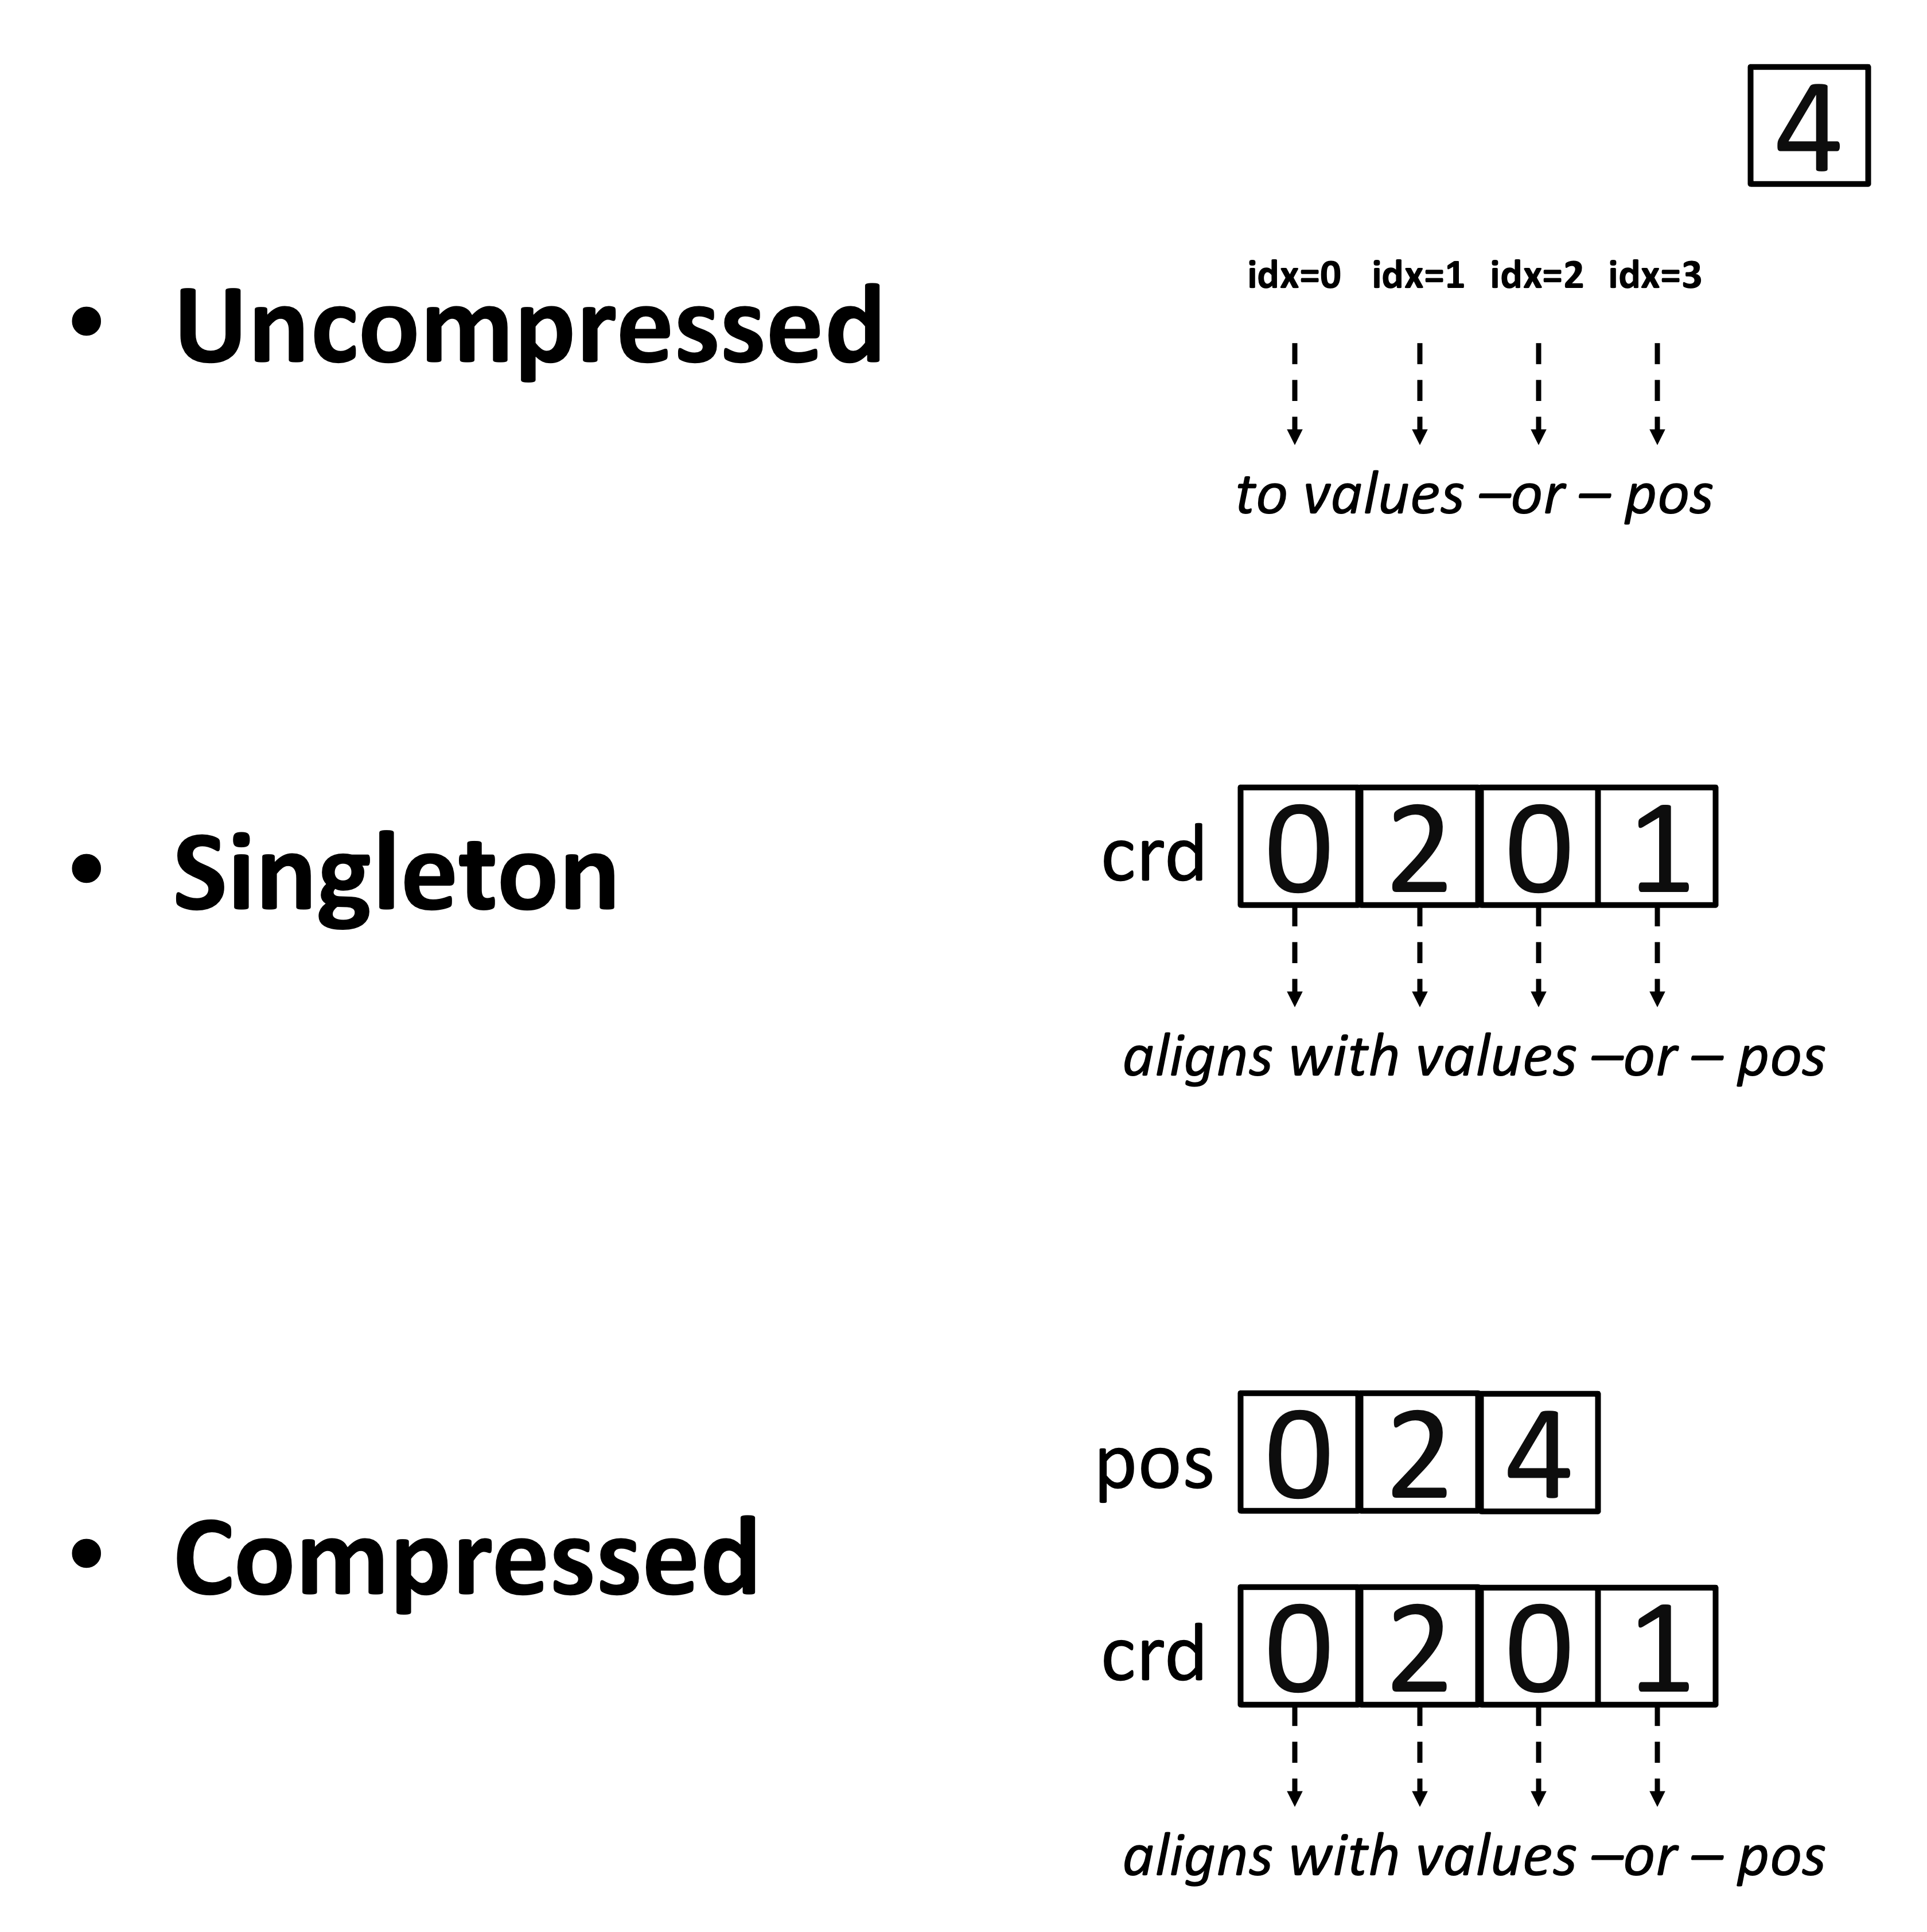
\includegraphics[width=0.5\textwidth]{figures/taco_levels.png}
\caption{A subset of TACO\cite{taco_format} \textit{level formats.}}
\label{fig:taco_levels}
\end{figure}

\begin{figure}[H]
    \centering
    \begin{subfigure}[b]{0.4\textwidth}
        \centering
        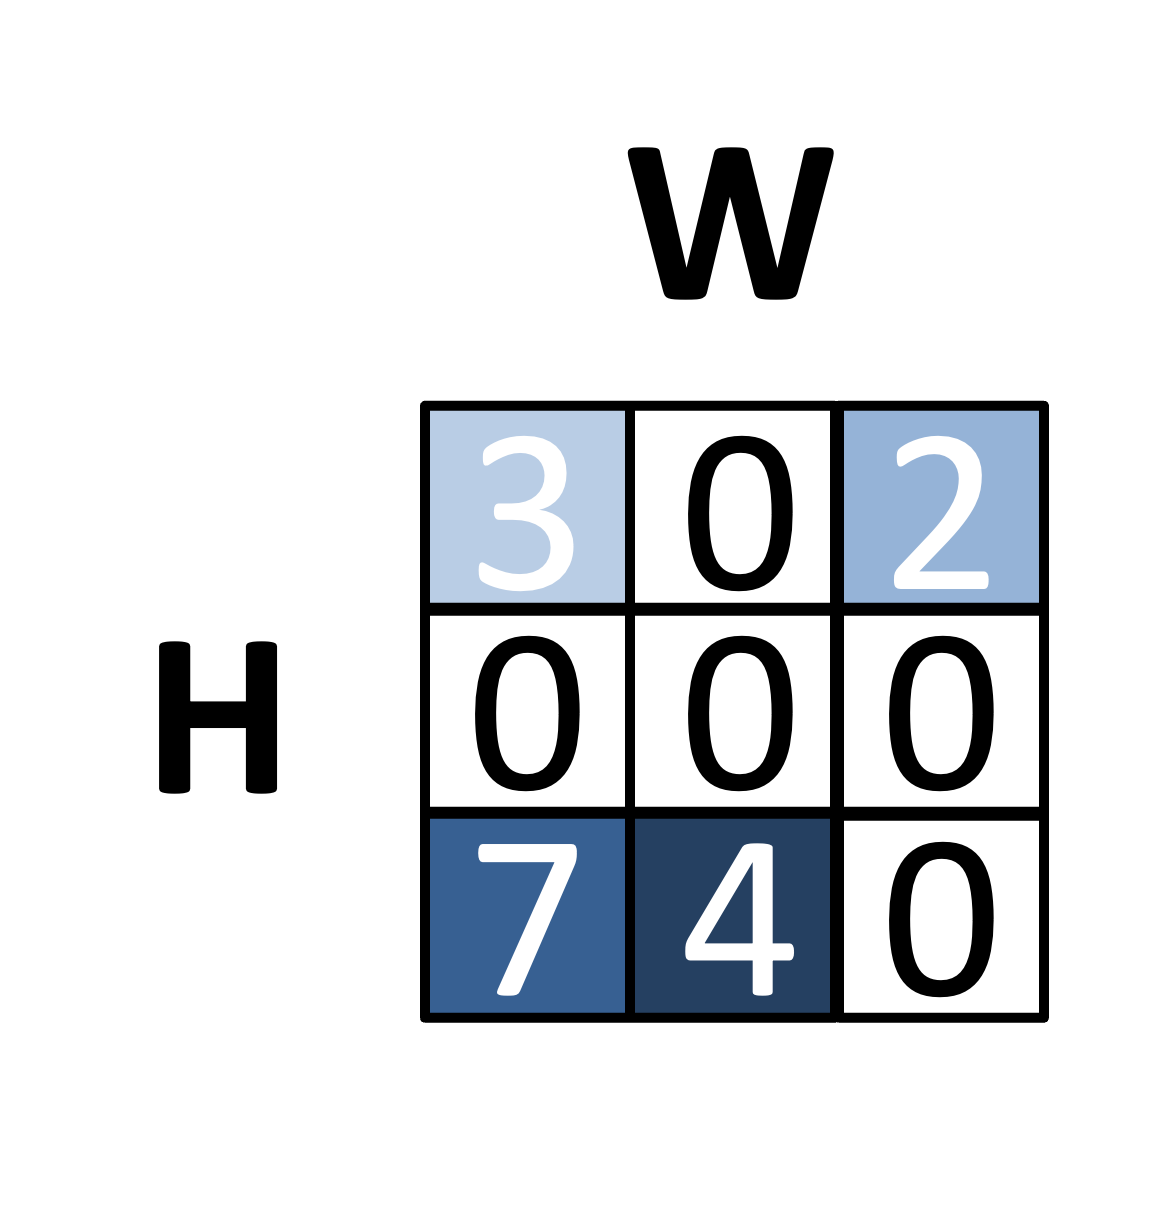
\includegraphics[width=\textwidth]{figures/taco_matrix.png}
        \caption{A 3x3 matrix.}
        \label{fig:taco_matrix}
    \end{subfigure}
    \hspace{0.5cm} % Adds space between the subfigures
    \begin{subfigure}[b]{0.4\textwidth}
        \centering
        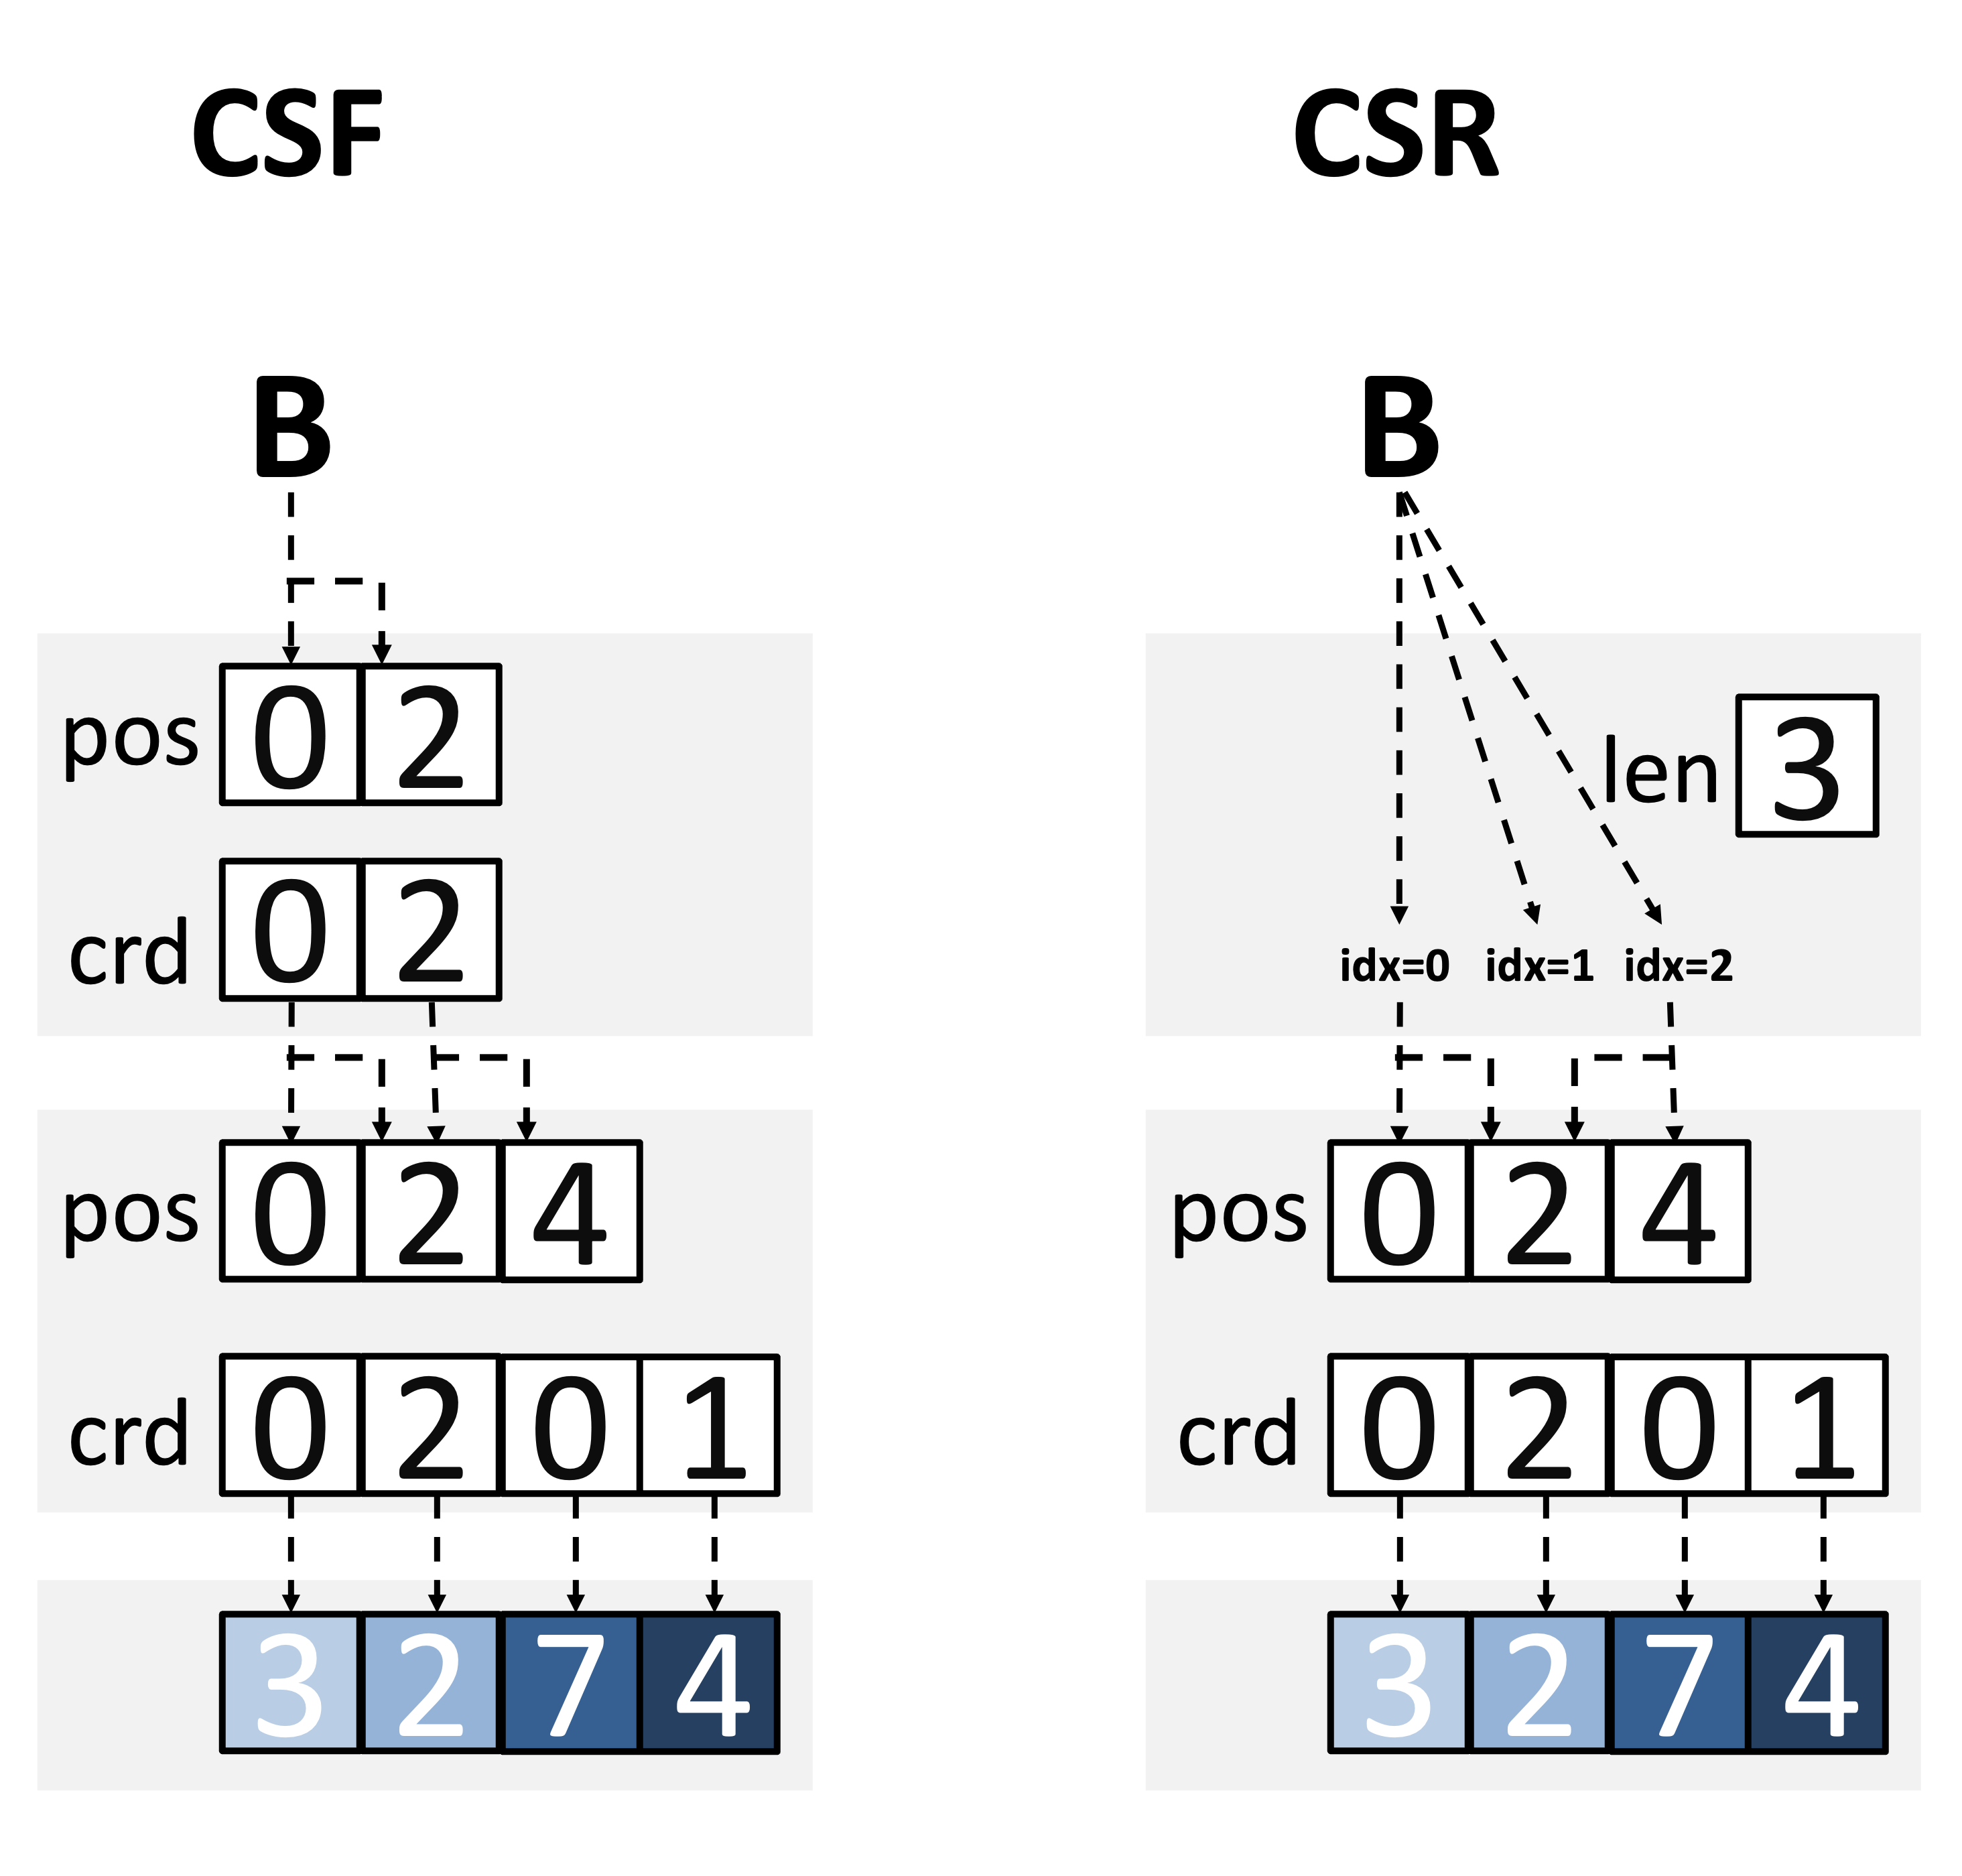
\includegraphics[width=\textwidth]{figures/taco_csf_csr.png}
        \caption{(\textit{left}) CSF format, expressed with TACO levels and level abstraction. (\textit{right}) CSR format, again expressed with TACO levels and level abstraction. The matrix from Figure~\ref{fig:taco_matrix} is used as a reference.}
        \label{fig:taco_csf_csr}
    \end{subfigure}
    \caption{Example of representing a matrix (2nd-order tensor) in both CSF and CSR formats, using level formats and level hierarchy from the TACO framework.}
\end{figure}

\begin{table}[h]
\centering
\caption{An excerpt from Table 1 of the TACO sparse format paper\cite{taco_format} showing the abstract interface to each TACO level format. V: supports coordinate value iteration.  P: supports position iteration. I: supports insert. A: supports append. (\checkmark) indicates that the particular property is contingent on the fiber configuration, whereas a normal checkmark indicates full support.}
\resizebox{\textwidth}{!}{%
\begin{tabular}{|l|ccc|ccccc|}
\hline
\textbf{Level Type} & \multicolumn{3}{c|}{\textbf{Capabilities}} & \multicolumn{5}{c|}{\textbf{Properties}} \\ 
& \textbf{Iteration} & \textbf{Locate} & \textbf{Assembly} & \textbf{Full} & \textbf{Ordered} & \textbf{Unique} & \textbf{Branchless} & \textbf{Compact} \\
\hline
Dense      & V & \checkmark & I & \checkmark & (\checkmark) & (\checkmark) & & \checkmark \\
Compressed & P & & A & (\checkmark) & (\checkmark) & (\checkmark) & & \checkmark \\
Singleton  & P & & A & (\checkmark) & (\checkmark) & (\checkmark) & \checkmark & \checkmark \\
\hline
\end{tabular}
}
\label{tab:taco_capabilities_properties}
\end{table}


\subsection{\textit{Efficient Processing}}

\textit{Efficient Processing of Deep Neural Networks}\cite{szebook} (Sze, Chen, et. al. 2020) (\textit{Efficient Processing} for short) introduced a number of abstractions for representing tensors in memory, for compressing tensor ranks, and for representing sparse dataflows. In practice the latter is closest to an existing taxonomy of SAF microarchitecture. 

\subsubsection{\textit{Efficient Processing} fibertree abstraction}

\begin{figure}[H]
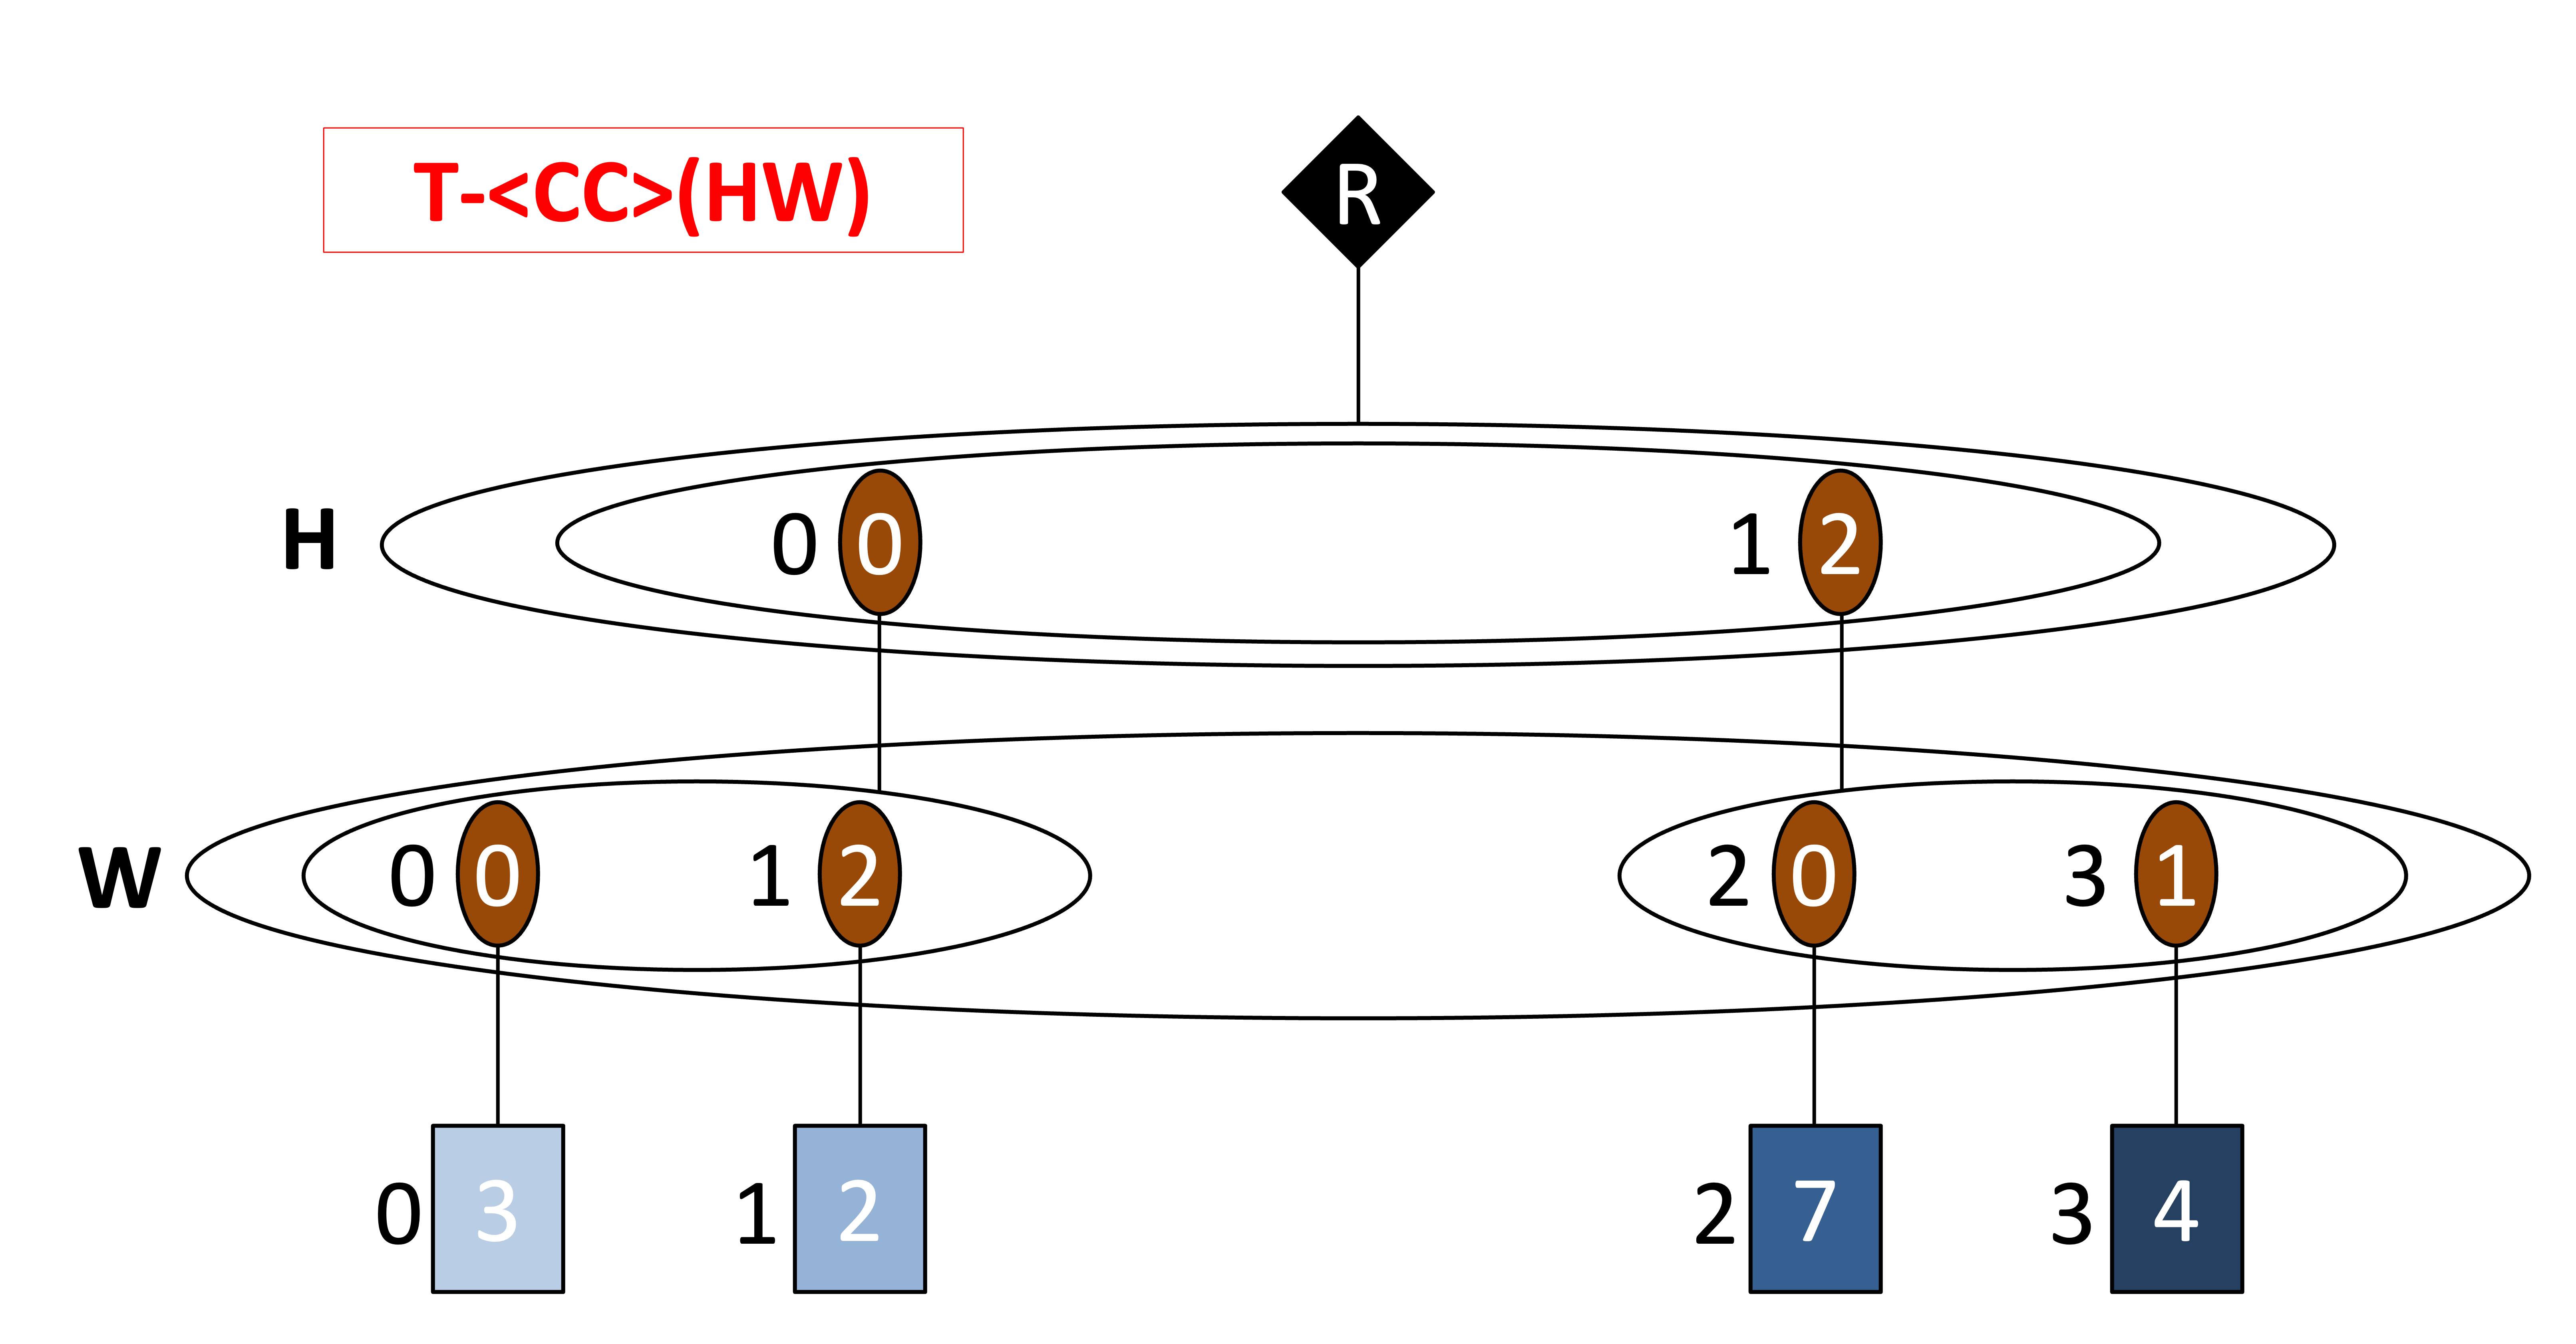
\includegraphics[width=\textwidth]{figures/efficient_processing_fibertree.png}
\caption{An example of the \textit{Efficient Processing} fibertree abstraction, applied to the matrix in Figure~\ref{fig:taco_matrix}.}
\label{fig:efficient_processing_fibertree}
\end{figure}



\textit{Efficient Processing} utilized the \textit{fibertree} abstraction for representing sparse tensors.

\paragraph{Parts of a fibertree.}

\paragraph{Tensor notation.}

\subsubsection{\textit{Efficient Processing} Taxonomy of representation formats}

\textit{Efficient Processing} introduced a taxonomy of sparse representation formats (from which Sparseloop\cite{sparseloop}
derived the Uncompressed, Coordinate-payload, Run-length-encoding, and Bitmask representation formats.) 

\subsubsection{\textit{Efficient Processing} Sparse dataflow \& SAF microarchitecture primitives}

Section 8.3 of \textit{Efficient Processing} introduced a framework for implementing ``sparse architecture dataflows''. The principle of this framework is that (1) the choice of sparse representation format frequently must be co-designed with SAF microarchitecture, however (2) it will be simpler to talk about sparse representation formats or SAF microarchitectures, respectively, if they each have decoupled representations; then co-design becomes effectively the cartesian product of possible sparse architectures and possible sparse format representations. 

Section 8.2 of \textit{Efficient Processing} already introduced fibertrees as a simple and intuitive abstraction for sparse representation formats, decoupled from the underlying microarchitecture. To that end, Section 8.3 of \textit{Efficient Processing} introduces two different abstractions for representing a sparse architecture dataflow which are decoupled from specific sparse representation formats:

\begin{itemize}
    \item \textbf{Dataflow as a loop nest.} Timeloop\cite{timeloop} represents dense architecture dataflows as loop nests which iterate \textit{by index} over coordinate values. \textit{Efficient Processing} introduces sparse loop nests, which extend Timeloop loop nest pseudocode with TACO\cite{taco_format}-style position iteration: each loop iteration uses Pythonic iterate-by-value syntax to get the next $(coord,pos)$ pair.
    \item \textbf{Dataflow as a topology built from a component taxonomy.} Once a sparse architecture dataflow is represented as a sparse loop nest, the aim of the \textit{Efficient Processing} framework is that this loop nest can be intuitively transformed to a microarchitecture topology. Based on the principle of decoupling format from dataflow, Section 8.3.1 of \textit{Efficient Processing} introduces a taxonomy of format-agnositic microarchitecture primitives. Each primitive is a either a memory, a sequence generator, a microarchitecture for comparing sparse format metadata streams, or some form of arithmetic. Each primitive has a set of ports associated with some datatype. These primitives are wired together into a topology which is animated by sequences of positions or coordinates from the sequence generators, thus implementing the sparse architecture dataflow.
\end{itemize}

\begin{figure}[H]
    \centering
    \begin{subfigure}[b]{0.2\textwidth}
        \centering
        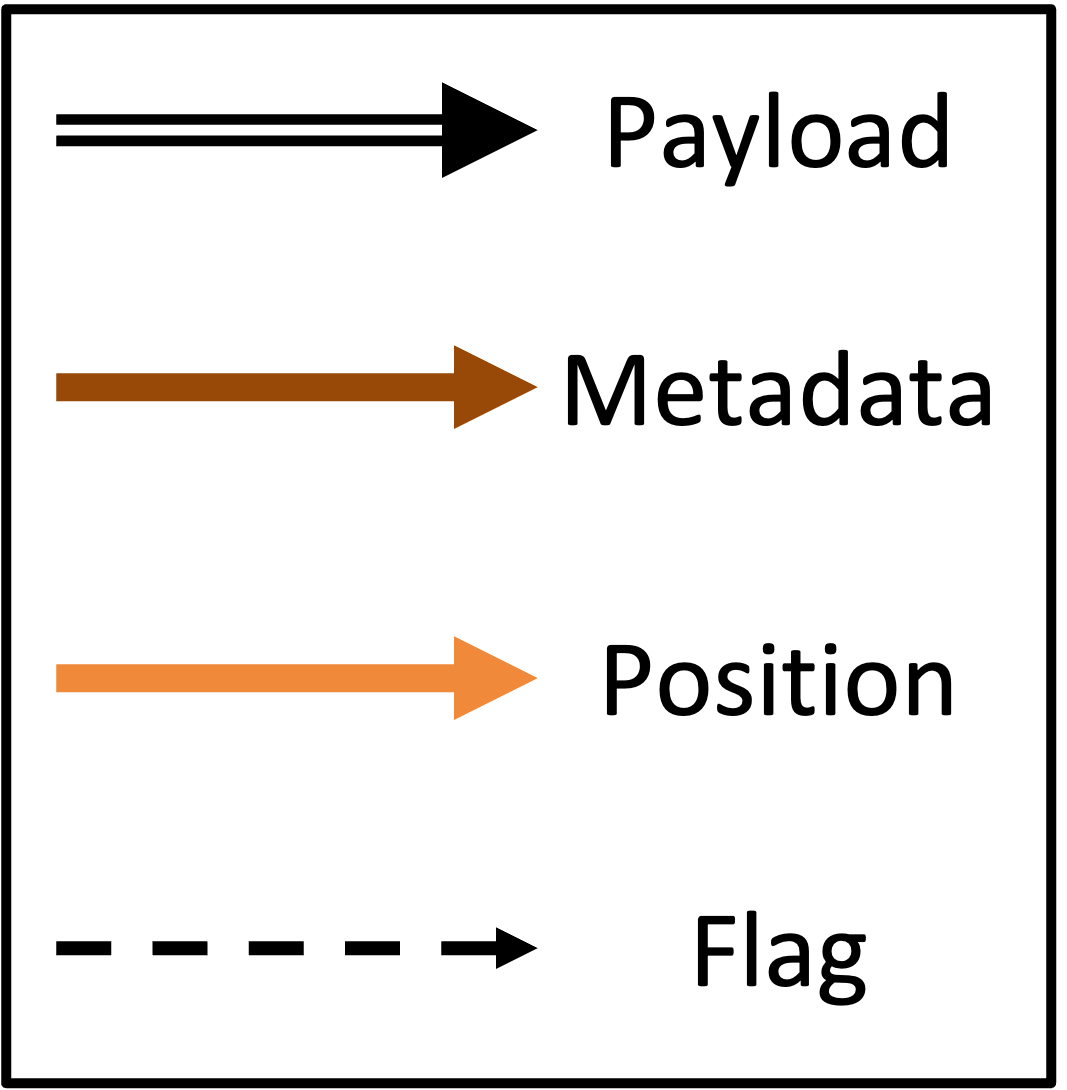
\includegraphics[width=\textwidth]{figures/efficient_processing_wire_legend.png}
        \caption{Wire types in the \textit{Efficient Processing} structural taxonomy for sparse architecture dataflows.}
        \label{fig:efficient_processing_wire_legend}
    \end{subfigure}
    \vspace{1cm} % Adds space between the subfigures
    \begin{subfigure}[b]{0.95\textwidth}
        \centering
        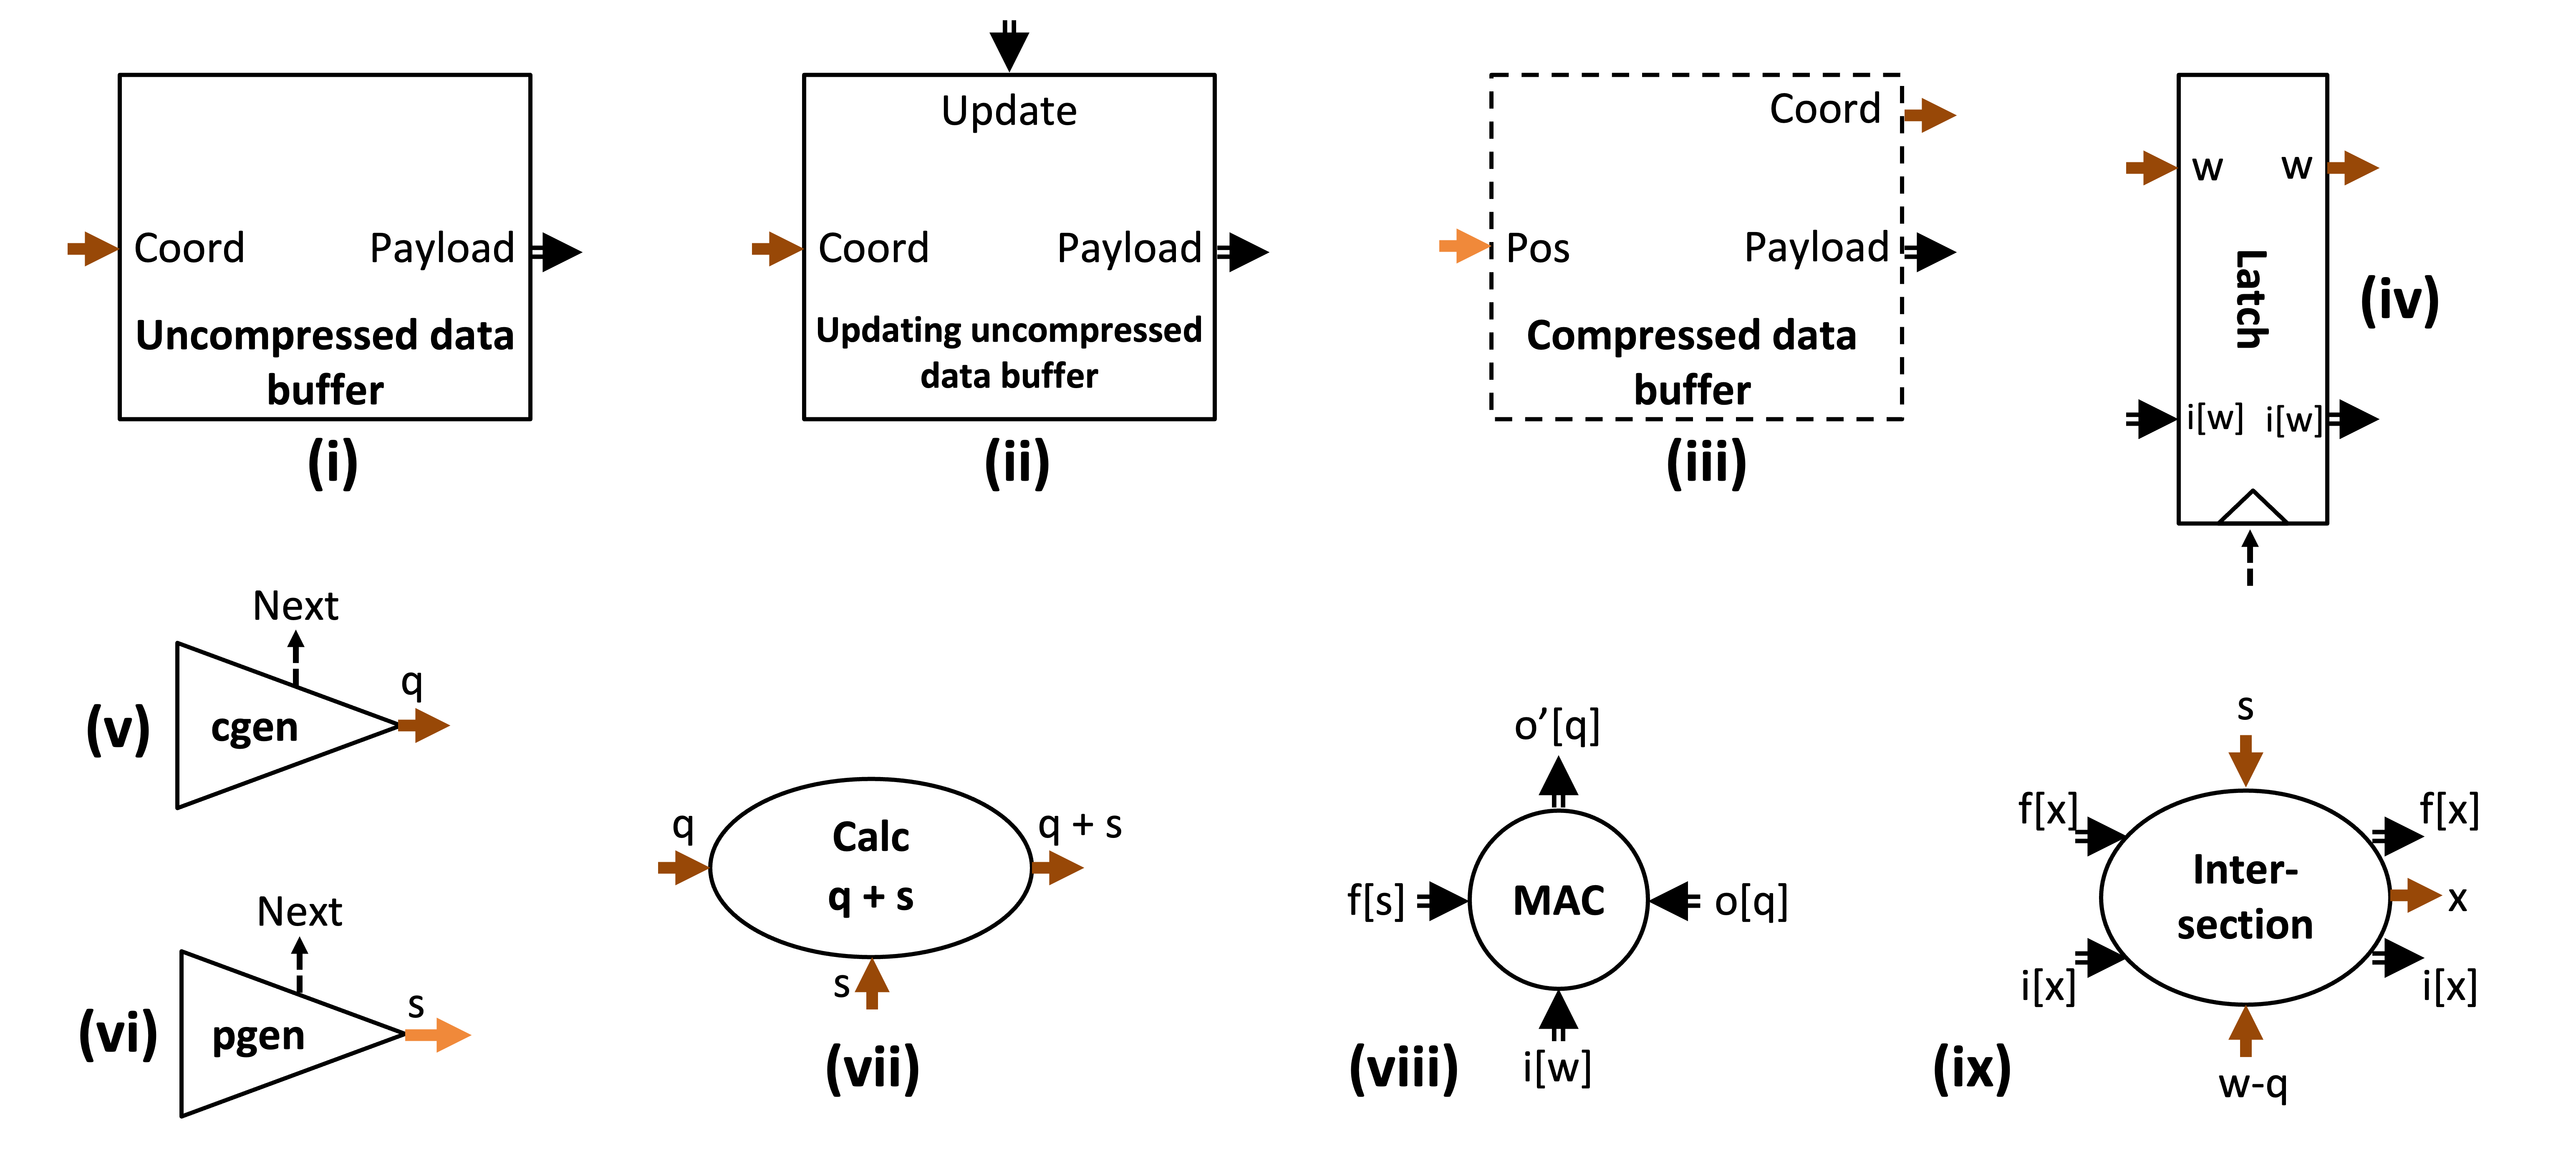
\includegraphics[width=\textwidth]{figures/efficient_processing_taxo.png}
        \caption{Components in the \textit{Efficient Processing} structural taxonomy for sparse architecture dataflows.}
        \label{fig:efficient_processing_taxo}
    \end{subfigure}
    \caption{Combined figure of wire types and components in the \textit{Efficient Processing} structural taxonomy.}
\end{figure}

Figure~\ref{fig:efficient_processing_wire_legend} and Figure~\ref{fig:efficient_processing_taxo} summarize the framework for building microarchitecture topologies. In this domain-specific framework, there are four types of wires (Figure~\ref{fig:efficient_processing_wire_legend}):

\begin{itemize}
    \item \textbf{Payload (black double-line) -} the data referenced by metadata; may comprise sub-tiles or individual data elements depending on the context of the larger design.
    \item \textbf{Metadata (brown single-line) -} a stream of sparse format metadata words.
    \item \textbf{Position (yellow-orange single-line) -} a stream of address offsets into architectural buffer memory (as distinct from coordinates which are offsets into dense coordinate space, and which are usually represented by brown metadata wires.)
    \item \textbf{Flag (dashed black line) -} a one-bit control signal, usually employed to synchronize control signals between components.
\end{itemize}

These are also the four possible port datatypes. There are nine primitives in this framework (Figure~\ref{fig:dense_smartbuffer_composition}):

\begin{itemize}
    \item \textbf{(i) Uncompressed data buffer -} a buffer with no sparse format optimization. Payloads are read by directly specifying coordinates as lookup addresses, which is possible because coordinates and positions are the same in a dense data structure. 
    \item \textbf{(ii) Updating uncompressed data buffer -} represents a buffer with support for both read and write (update) operations, and no format optimization.
    \item \textbf{(iii) Compressed data buffer - } a buffer with a sparse format representation. A payload and its associated memory data are selected by a positional input.
    \item \textbf{(iv) Latch - } Single architectural register for holding a datatype stationary.
    \item \textbf{(v) Coordinate generator - } Sequence generator for abstract coordinates.
    \item \textbf{(vi) Position generator - } Sequence generator for address offsets in memory.
    \item \textbf{(vii) Coordinate calculator - } small, low-cost arithmetic unit which is required to implement the projection expressed by the problem dataspace.
    \item \textbf{(viii) Multiply Accumulate Unit (MAC) - } Compute.
    \item \textbf{(ix) Intersection unit - } Stand-in for a variety of components which select pairs of operand payloads based on an inner join on coordinate metadata.
\end{itemize}

As a way of illustrating different sparse dataflows, Section 8.3 of \textit{Efficient Processing} expresses a number of contemporary sparse tensor accelerator designs (\cite{cambricon_x}\cite{cnvlutin}\cite{scnn}\cite{sparten}\cite{eyerissv2}\cite{eie}\cite{extensor}), first in sparse loop nest form, and then as microarchitecture topologies which implement the sparse loop nests.

\subsection{Sparse abstract machine}

\subsection{Sparseloop}

Sparseloop\cite{sparseloop} developed a unified taxonomy of Sparse Acceleration Features (SAFs), architectural optimization strategies for exploiting sparsity (zero-sparsity) to conserve energy and cycles. A SAF is a strictly declarative description of an optimization, comprising (1) a description of the optimization outcome (i.e. skipping of certain compute operatinos), (2) a set of attributes which modulate the outcome of the optimization, and (3) a binding to a particular architectural buffer or compute component. A SAF describes neither the microarchitectural implementation of the optimization, nor the interfaces or communication protocols involved in integrating the microarchitectural implementation into the design. 

Nonetheless, a real design would require a microarchitectural change which implements the optimization, referred to here as the \textit{SAF microarchitecture.} Existing analytical modeling tools\cite{sparseloop} model only the benefits of exploiting SAFs (savings on memory capacity, fewer memory accesses, fewer compute cycles); these benefits are introduced in Section~\ref{background:safs}. These tools avoid modeling the costs of SAF microarchitectures by assuming (1) an ideal SAF microarchitecture which perfectly implements the SAF, and (2) a SAF microarchitecture with negligible energy and area overhead.

Section~\ref{background:safs} the Sparseloop unifed SAF taxonomy. Section~\ref{background:saf_uarch} demonstrates that SAF microarchitectures can \textit{sometimes} have significant implications for the design and modeling of sparse tensor accelerators. Thus, this work is motivated by the need to create novel SAF microarchitecture models.

%
% SAFs subsection
%
\subsubsection{SAFs}
\label{background:safs}

This section will review and motivate the two broad SAF categories. Table~\ref{tab:design_specific_models} provides examples of how SAFs are used in prior research.

%
% Figure: examples of action optimizations
%
\begin{figure}[H]
\includegraphics[width=\textwidth]{figures/saf_action_optimizations.PNG}
\caption{An example of dot-product optimized with zero-gating and zero-skipping to save cycles and energy, versus the naive un-optimized approach. The zero-skipping optimization's efficacy may depend on the choice of leader-follower skipping vs bidirectional skipping.}
\label{fig:saf_action_optimizations}
\end{figure}
%
% Table: Action SAFs, comparison of perf and energy
%
\begin{table}[ht]
\begin{tabular}{c|c|c|}
 & Cycles & Energy \\ \hline \hline
Theoretical &  \textcolor{green}{\textbf{1}} & \textcolor{green}{\textbf{$E_{mac}$}}\\ \hline
Naive &  \textcolor{red}{\textbf{5}} & \textcolor{red}{\textbf{$5 E_{mac}$}}\\ \hline
Zero-gating &  \textcolor{red}{\textbf{5}} & \textcolor{green}{\textbf{$E_{mac}$}} \\ \hline
Zero-skipping (leader-follower) & \textcolor{red}{\textbf{2}} & \textcolor{red}{\textbf{$2 E_{mac}$}} \\ \hline
Zero-skipping (bidirectional) & \textcolor{green}{\textbf{1}} & \textcolor{green}{\textbf{$E_{mac}$}} \\ \hline
\end{tabular}
\caption{Dot-product cycles and energy with different action-optimization strategies applied to the PE in Figure \ref{fig:saf_action_optimizations}, versus the theoretical-best. Energy is measured in multiples of the energy of a single MAC, $E_{mac}$}
\label{tab:action_saf_comparison}
\centering
\end{table}
%
% Content: SAFs
%
\paragraph{Action optimizations.} These are SAFs which signify that the tensor accelerator detects and optimizes away ineffectual operations such as $0 \times 0 = 0$ and $0 \times a = 0$, with the goal of saving energy and potentially compute cycles. Figure \ref{fig:saf_action_optimizations} compares action optimization cost for a dot-product problem mapped to a simple PE with two buffers and a MAC unit which consumes $E_{mac}$ per operation. Theoretically only one cycle and $E_{mac}$ energy should be required to multiply $a_0 \times b_0$; there are no other effectual MAC operations. Table \ref{tab:action_saf_comparison} shows that a "naive" PE design with no action optimization SAFs underperforms on both cycles and energy by $5\times$, and Figure \ref{fig:saf_action_optimizations} shows that the cause is ineffectual MACs being performed. \textit{Zero-gating} (or \textit{gating}) conserves $E_{mac}$ energy per ineffectual MAC since the MAC unit idles for a cycle. In other words there is no conservation of cycles for ineffectual operations, only energy. \textit{Zero-skipping} (or \textit{skipping}) conserves $E_{mac}$ per ineffectual MAC, but does so by skipping immediately to the next one - thus both energy and time are saved by skipping. 

Designs with \textit{bidirectional action optimizations} do not perform a MAC when either operand is zero. Thus 100\% of gating or skipping opportunities are exploited, depending on the type of action optimization. Designs with \textit{leader-follower action optimizations} respond only to the designated leader operand being zero, in which case both the MAC and the follower memory access are skipped or gated.

Figure~\ref{fig:saf_action_optimizations} summarizes the attributes of action optimizations. The key attribute for both skipping and gating action optimizations is direction (\textit{bidirectional} vs \textit{leader-follower}.)

%
\paragraph{Format optimizations.} The zero-compression (or \textit{format}) SAF discards ineffectual zero-valued tensor elements in order to save memory capacity at rest and memory bandwidth during acceses. The remaining nonzero values' positions in memory no longer align with the original coordinates, so the compressed format requires metadata which may be used to recover an element's uncompressed coordinate as efficiently as possible (Figure \ref{fig:saf_format_optimizations}.) 

The three representation formats studied in this work are

\begin{itemize}
    \item \textbf{Uncompressed (U)} - U represents a vector as it exists in memory without any compression, including zero-value elements. The sparse tensor architectures which we consider here, will typically eschew U in favor of a compressed format.
    \item \textbf{Uncompressed Offset Pairs (UOP)} - UOP 
    \item \textbf{Coordinate Payload (C)}
    \item \textbf{Bitmask (B)}
\end{itemize}

These are derived from the Sparseloop\cite{sparseloop} paper.

%
% Figure: examples of format optimizations
%
\begin{figure}[H]
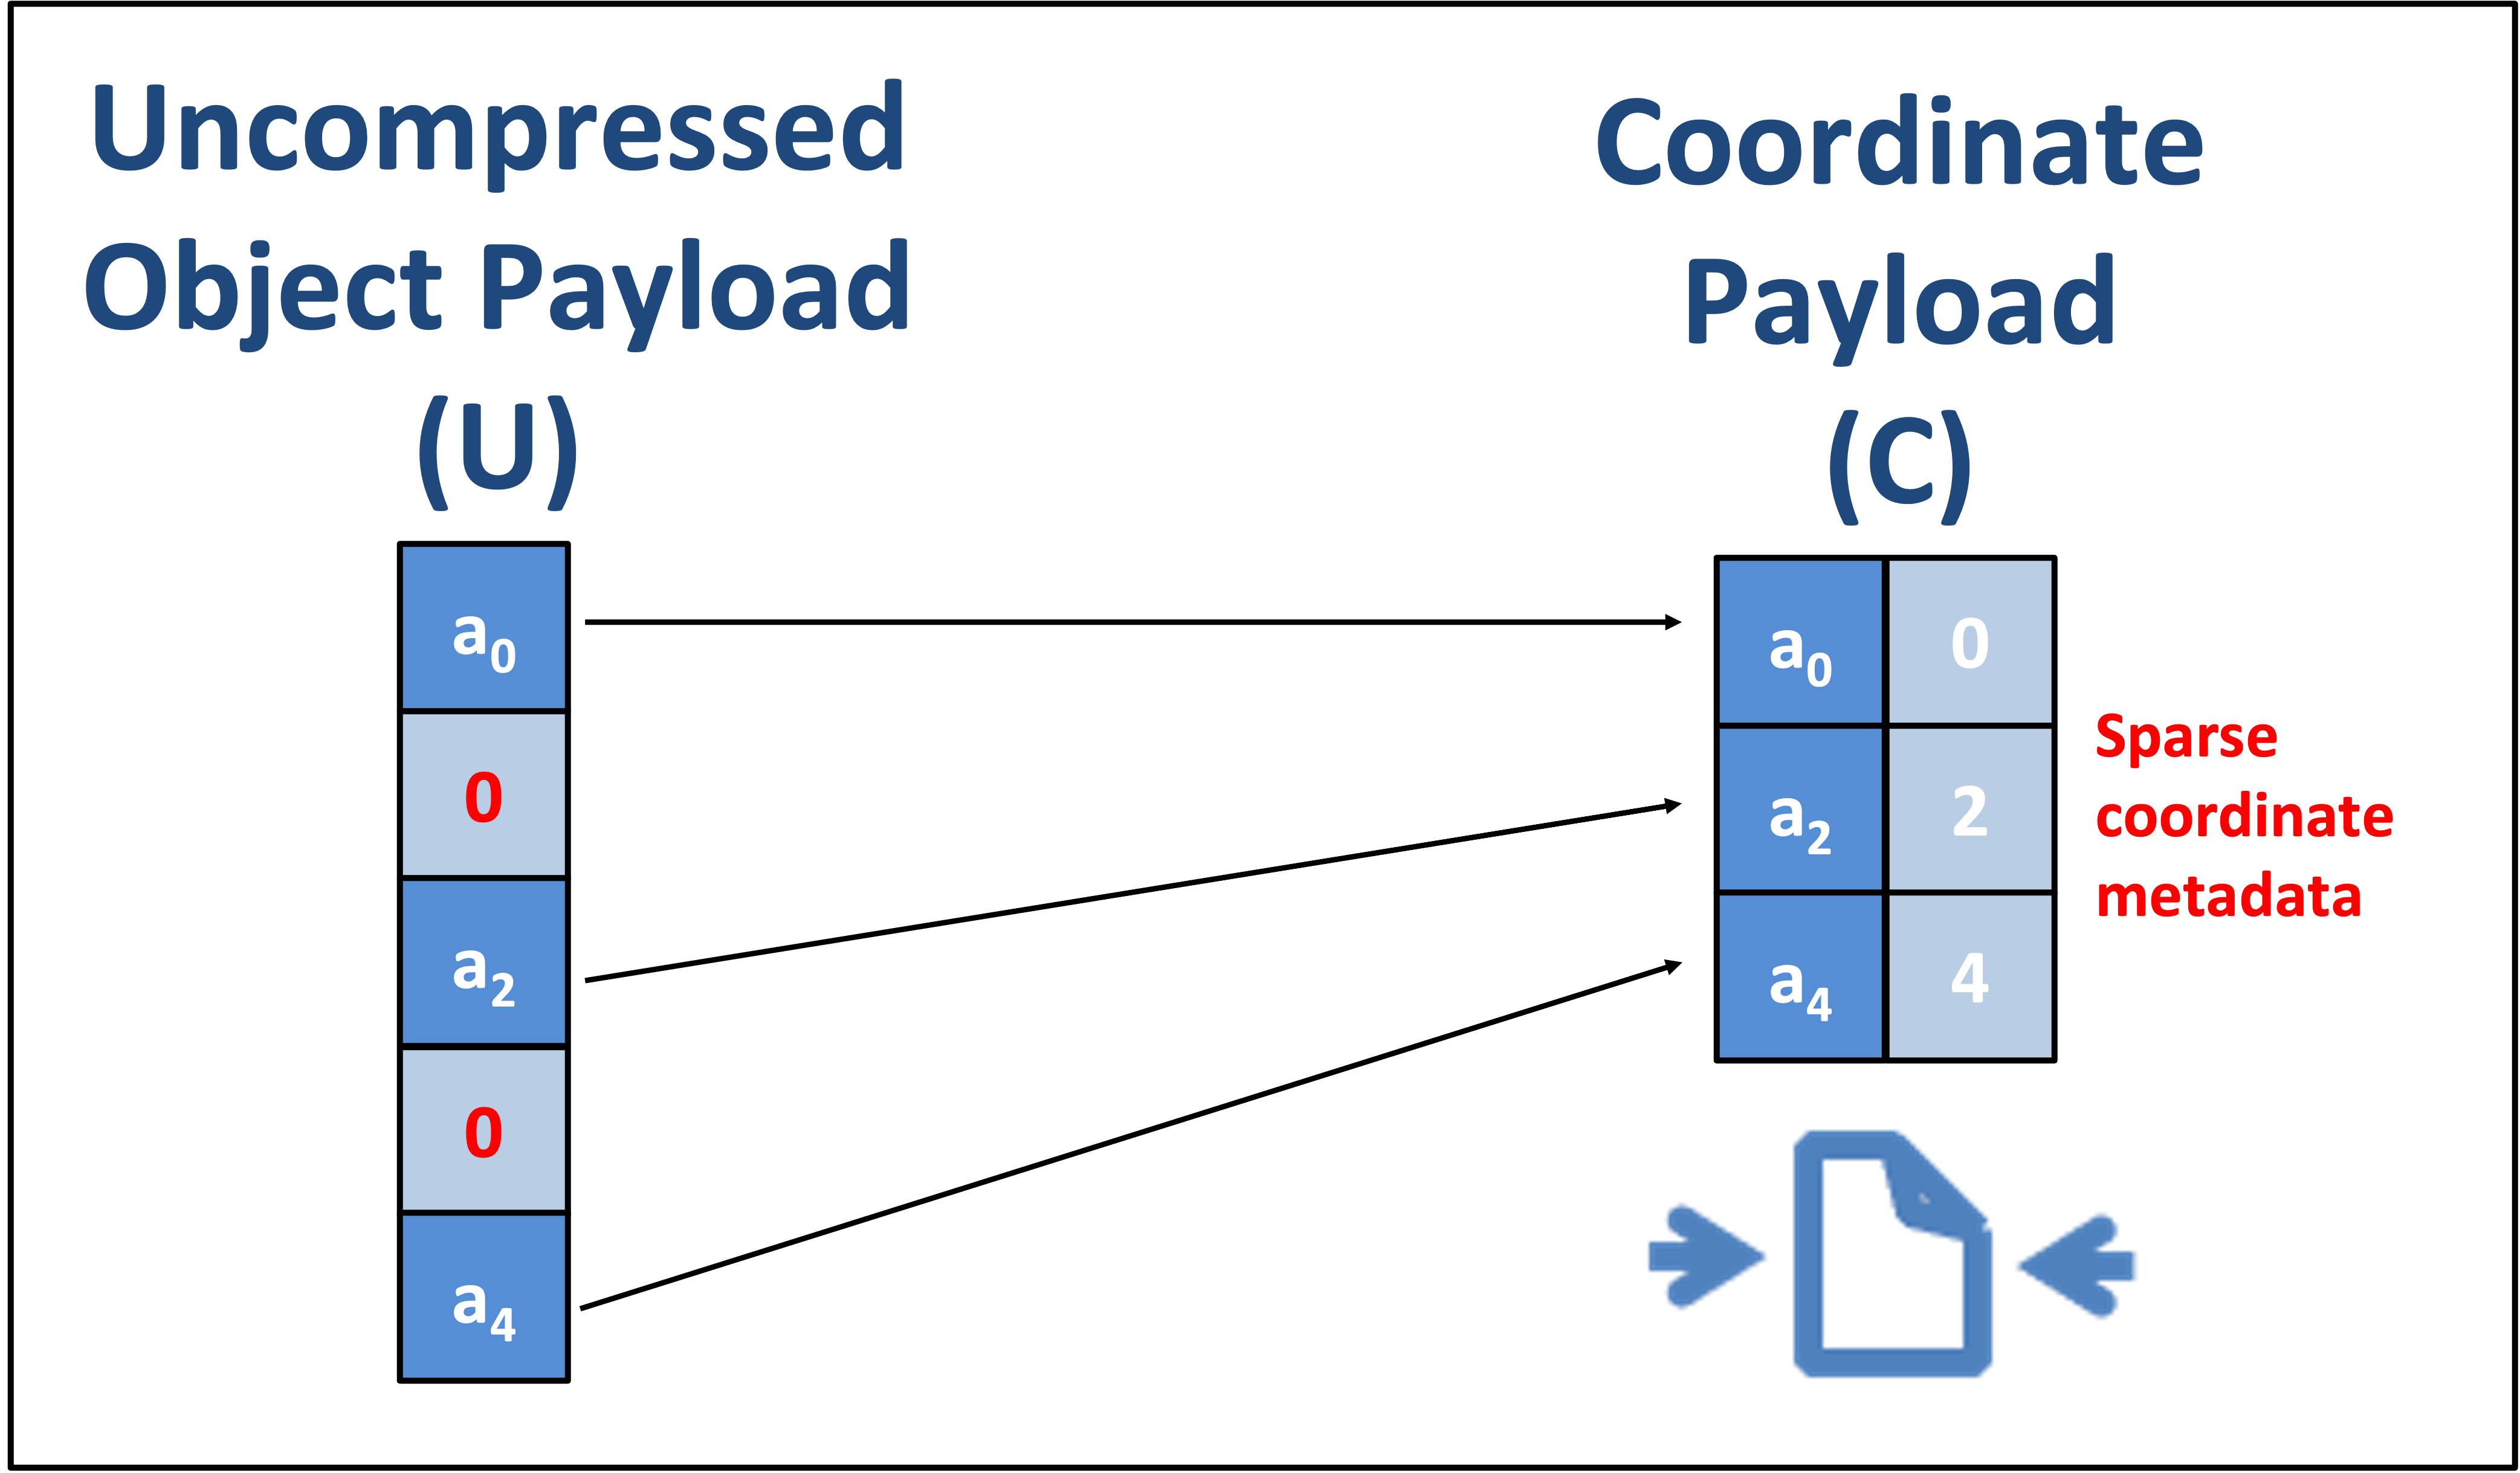
\includegraphics[width=8cm]{figures/saf_format_optimizations.PNG}
\caption{A visualization of a compressed representation format (coordinate-payload or CP) applied to a vector with some zero entries. The compressed representation is reduced to nonzero values and metadata which recovers the original data structure.}
\label{fig:saf_format_optimizations}
\end{figure}
%
% Content: format optimizations
%

%
% Figure: combined action/format optimizations
%
\begin{figure}[H]
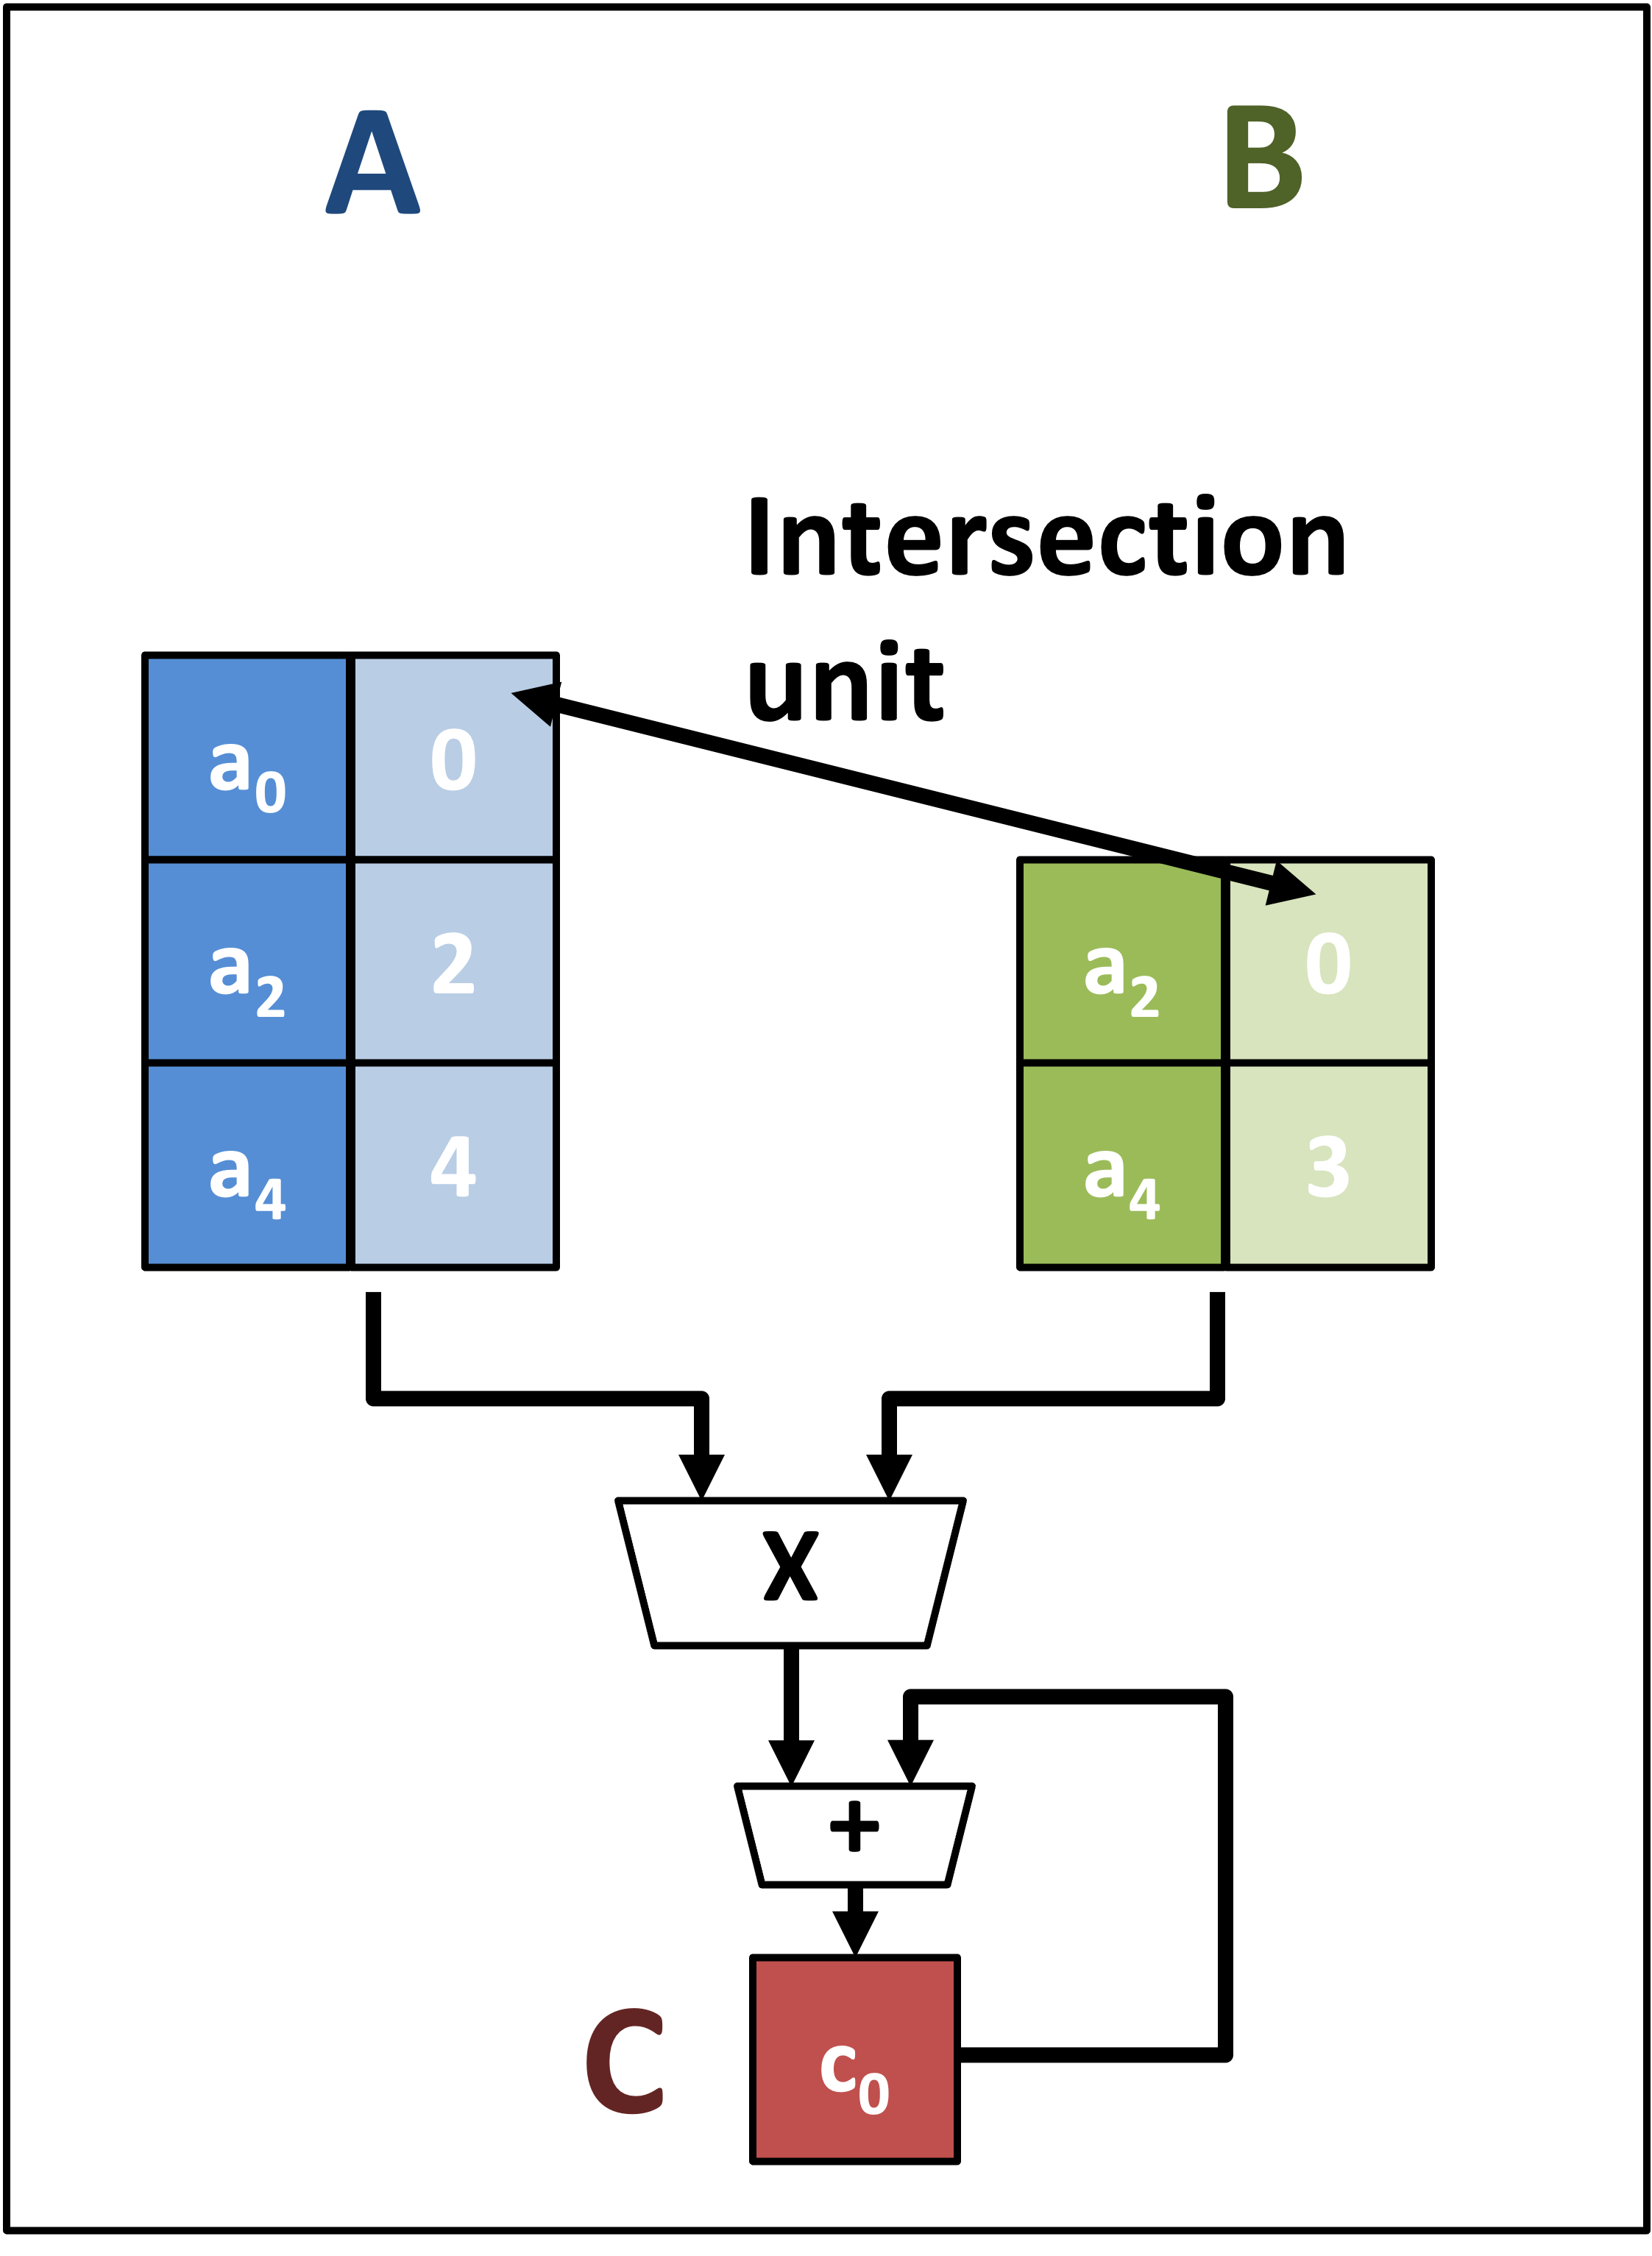
\includegraphics[width=4cm]{figures/saf_action_format_combo.PNG}
\caption{An example of dot-product optimized with both bidirectional zero-skipping and a compressed representation format. Conceptually corresponding nonzero values must be matched using a component which processes format metadata in order to implement skipping, which is called an \textit{intersection unit.} The cost of the skipping optimization is the energy, area and latency of the skipping microarchitecture, which comprises the intersection unit.}
\label{fig:saf_action_format_combo}
\centering
\end{figure}

\subsubsection{Sparseloop workflow}

\begin{figure}[H]
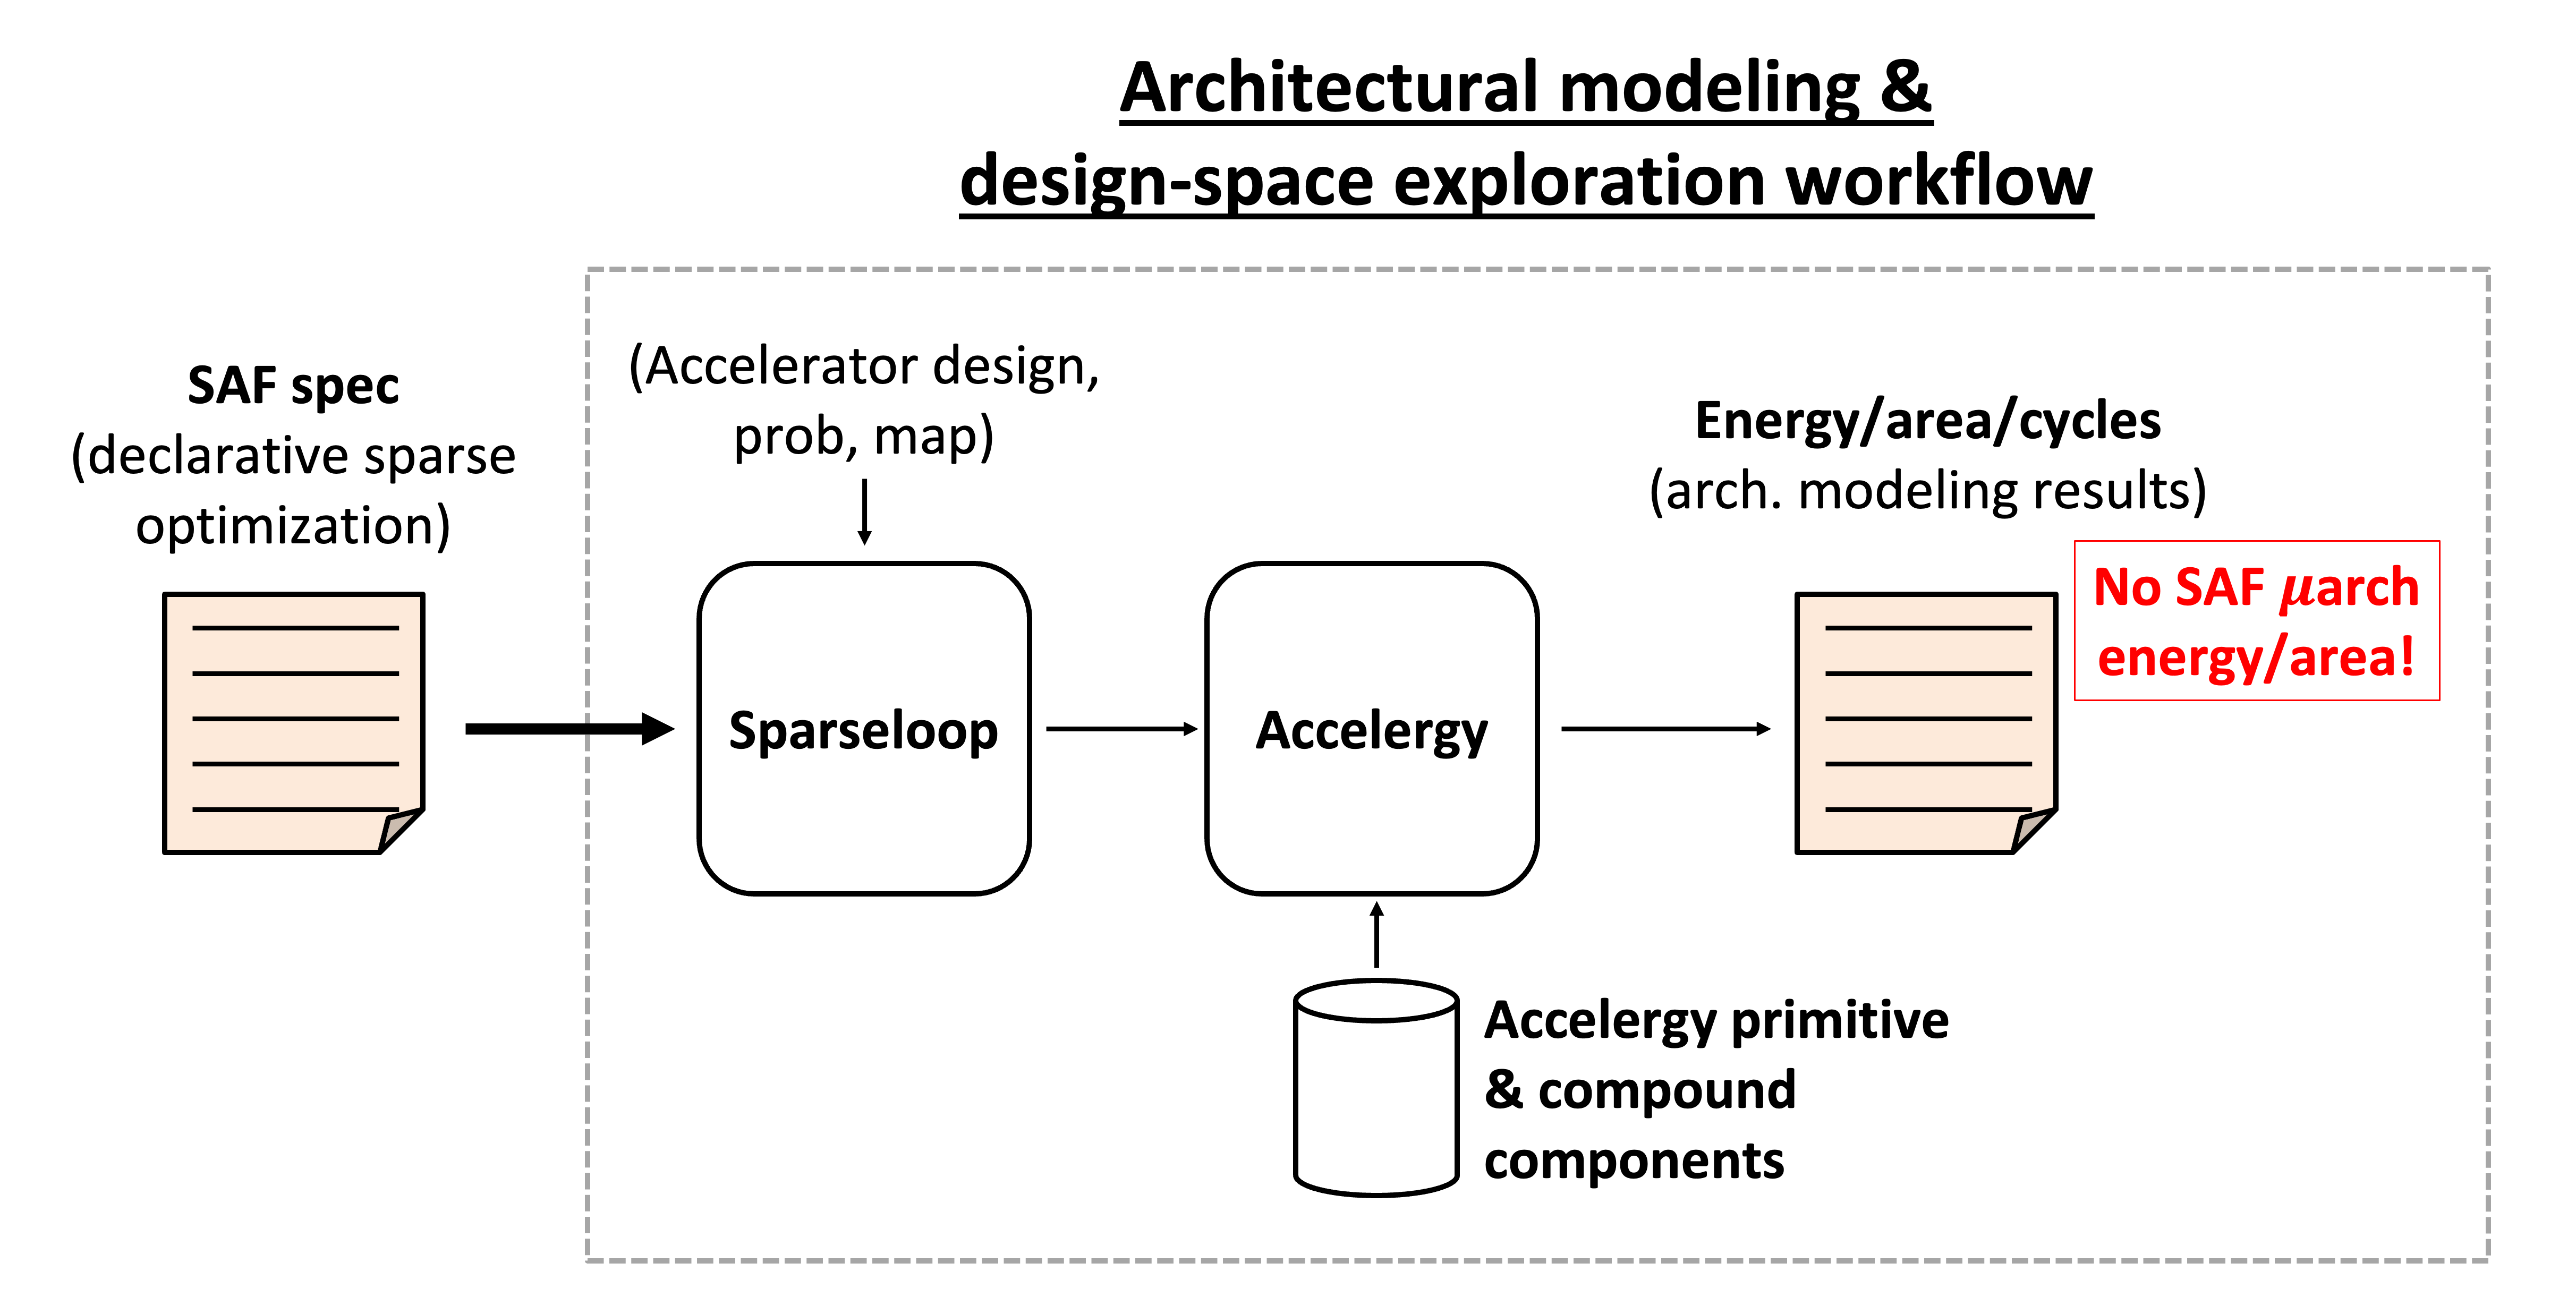
\includegraphics[width=8cm]{figures/sparseloop_workflow.png}
\caption{The Sparseloop workflow for architectural modeling and design-space exploration, simplified.}
\label{fig:sparseloop_workflow}
\end{figure}

\section{SAF microarchitectures}
\label{background:saf_uarch}
%
% Figure: SAFs can be significant or not, it depends on the microarchitecture
%
\begin{figure}[H]
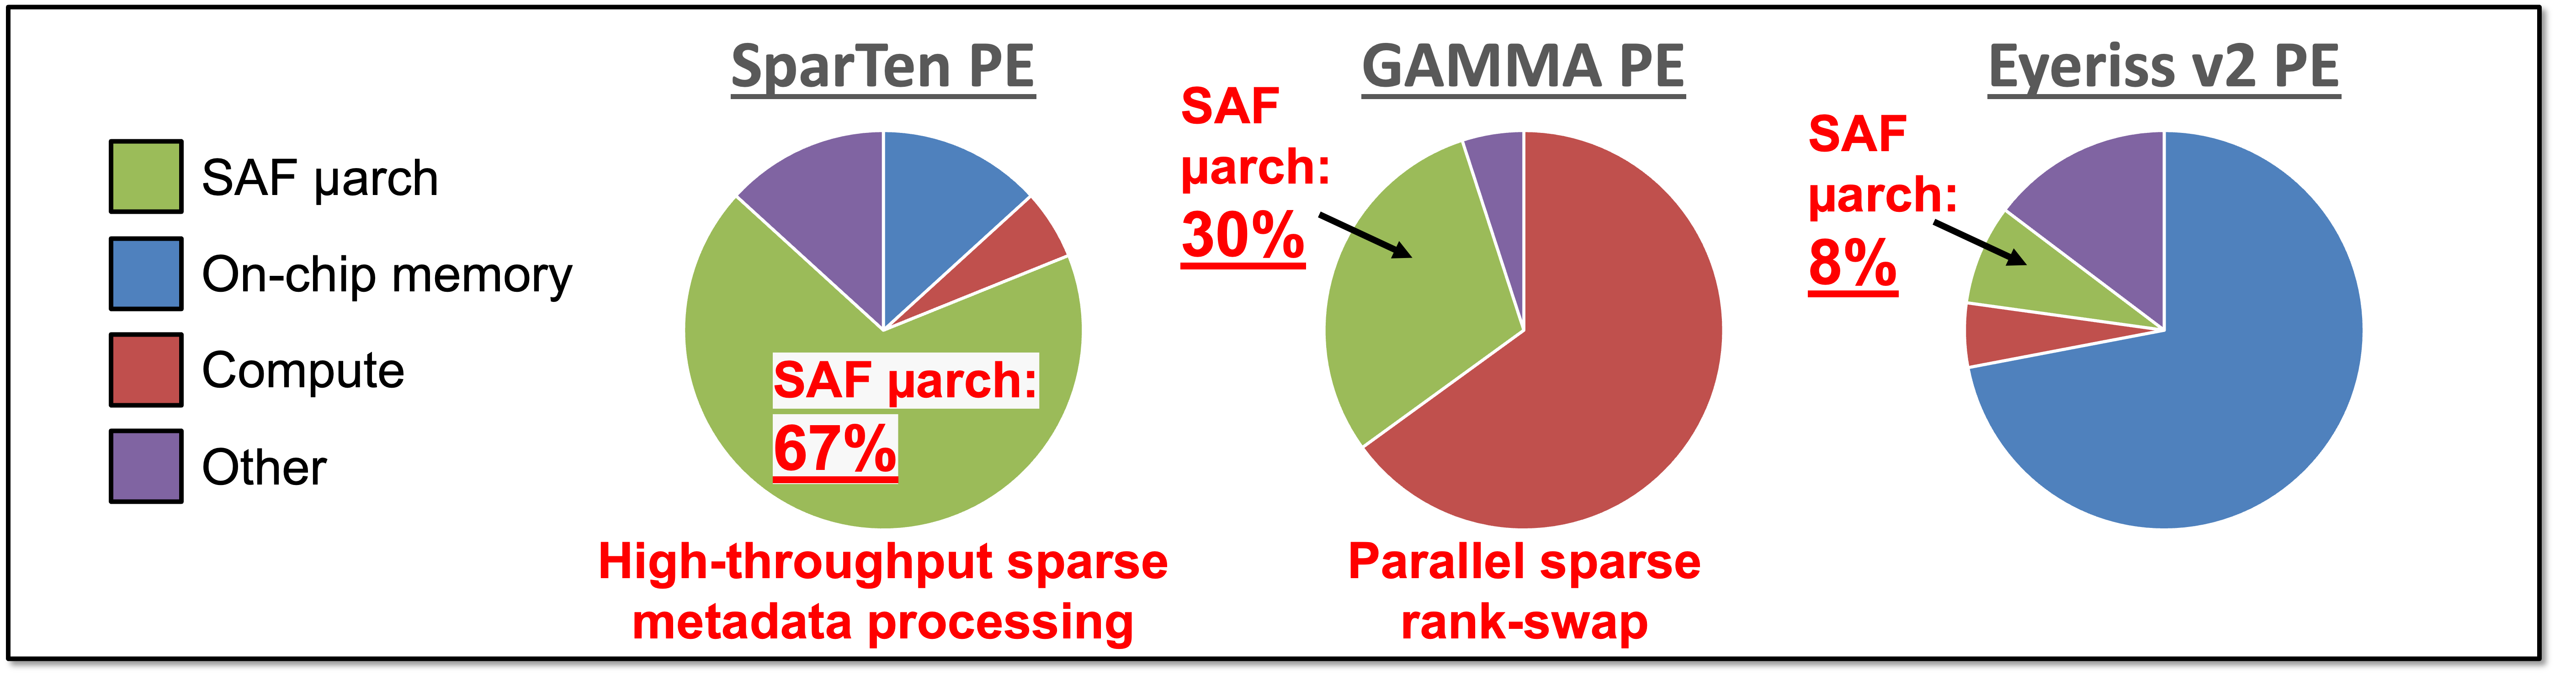
\includegraphics[width=\textwidth]{figures/saf_uarch_significance.PNG}
\caption{Breakdown of sparse tensor accelerator PE area based on published RTL simulations for a representative sample of designs. The total area of PE architectural components is a decent model of Eyeriss v2\cite{eyerissv2} PE area because Eyeriss v2's simple leader-follower zero-skipping microarchitecture has negligible area. SparTen\cite{sparten} employs a complex zero-skipping microarchitecture which must process high-throughput bitmask metadata. GAMMA's\cite{gamma} PE coordinates loop-nest re-ordering with tensor layout shuffling while the data is in-flight, using a high-radix merger component. These complex microarchitectures create discrepancies against architectural PE models.}
\label{fig:saf_uarch_significance}
\centering
\end{figure}

Prior research on sparse tensor acclerators proposes many different SAF microarchitectures, without employing a consistent set of abstractions and models in order to explore the design space or make comparisons. However, the breakdown of PE area for several accelerator designs in Figure~\ref{fig:saf_uarch_significance} shows that it is not always safe to assume SAF microarchitecture overhead is insignificant, and so it is important to choose SAFs and SAF microarchitecture designs systematically to minimize cost.

The Eyeriss v2\cite{eyerissv2} PE implements a leader-follower skipping SAF, devoting only 8\% of its PE area to the skipping microarchitecture. This is owing to a lightweight leader-follower skipping microarchitecture which operates on sparse weights and activations in Compressed-Sparse Column (CSC) format. 

In contrast, the SparTen\cite{sparten} accelerator PE uses most of its PE area for the bidirectional skipping microarchitecture which operates on Bitmask-format metadata. As will be shown later, this is attributable to the substantial load-handling capability which the skipping microarchitecture must have in order to maintain high arithmetic hardware utilization. 

As a final example, the GAMMA\cite{gamma} accelerator PE devotes 30\% of its PE area - a significant amount - in order to apply a rank swap\footnote{Rank swap refers to transposing tensor rank traversal order, as described in\cite{sparse_arch_lecture1}.}. The PE employs a row-wise product dataflow for loading CSR-format GEMM ($C_{M\times N} = A_{M\times K} \times B_{K\times N}$) operands from memory. A single $A_{M\times K}$ element and a row of $B_{K\times N}$ elements are loaded from on-chip memory into the PE; this reflects that the $N$ rank of B is traversed in the inner-most loop, while the contracted $K$ rank is traversed at an intermediate loop level. Row-wise product enables a cheap leader-follower skipping microarchitecture to be employed for loading $B_{K\times N}$ rows conditional on non-zero $A_{M\times K}$ elements. Upon receiving $A_{M\times K}$ and $B_{K\times N}$ values from memory, the GAMMA PE implements a rank-swap which moves the contracted dimension $K$ into the innermost loop. This enables inner-product accumulation into a single PE output register. The output memory footprint saved by the rank-swap is significant: a design such as MatRaptor\cite{matraptor} which implements row-wise product \textit{without} a rank-swap must store and incrementally accumulate $|K|$ rows of partial outputs, each of size $1 \times |N|$, requiring increased output memory footprint. Given the benefit of rank-swap, is there a tradeoff involved in using it? The use of CSR in GAMMA, means thank rank-swap requires a merge primitive (analogous to the merge operation in mergesort) in order to do a stable sort of $B_{K\times N}$ operand data by $K$ coordinate metadata, effectively implementing a transpose. GAMMA employs a radix-64 merge unit\cite{gamma} in order to do this. Although the rank-swap itself is not a sparse optimization, nonetheless the need for this type of merge unit results from employing a rank-swapped dataflow \textit{in the context of employing CSR format for the $B_{K\times N}$ operand}. Thus it is justifiable to say that the merge unit is part of the format microarchitecture which implements the CSR format SAF. It is this format microarchitecture which accounts for 30\% of PE area in GAMMA.

Clearly, SAFs and SAF microarchitecture designs are complex and impactful design decisions, and it is desirable to know whether a particular combination of SAFs will lead to the substantial PE implementation overhead seen (for example) in SparTen and GAMMA. The rest of this work develops a conceptual framework for taxonomy and modeling of SAF microarchitectures. This conceptual framework can be represented in software and utilized to make SAF microarchitecture design decisions using analytical pre-RTL modeling tools.

\subsection{Existing SAF microarchitecture designs}

%
% Figure: prior work
%
\begin{table}[ht]
\begin{tabular}{c|c|}
\textbf{Accelerator} & \textbf{SAF microarchitecture proposals} \\ \hline \hline
Eyeriss &  MAC gating; in-flight RLE decompression \\ \hline
Eyeriss v2 & CSC zero-skipping \\ \hline
ExTensor & Hierarchical bidirectional zero-skipping \\ \hline
SCNN & Memory conflict handling (binning output coordinates) \\ \hline
SparTen & Bitmask zero-skipping, parallel compression, memory conflict handling \\ \hline
OuterSPACE & Software rank-swap \\ \hline
GAMMA & Leader-following intersection, hardware rank-swap \\ \hline
\end{tabular}
\caption{A non-exhaustive list of published tensor accelerators and their proposed SAF microarchitectures.}
\label{tab:design_specific_models}
\centering
\end{table}

